\documentclass[12pt]{pom_thesis}
\usepackage[T1]{fontenc}
\input{commands_packages}
\usetikzlibrary{decorations.pathreplacing,angles,quotes}
\usepackage{mathrsfs}
\usepackage[euler-digits]{eulervm} %TODO: Maybe change this
\author{Leo Selker}
\advisor{Vin de Silva}
\title{M\"obius Inversion: Construction and Applications}
\newcommand{\fix}{\text{fix }}
\newcommand{\cl}{\text{cl }}
\DeclareMathOperator{\cat}{cat}
\DeclareMathOperator{\ps}{\mathscr{P}}
\DeclareMathOperator{\sub}{Sub}
\DeclareMathOperator{\stab}{Stab}
\DeclareMathOperator{\orb}{Orb}
\DeclareMathOperator{\fixx}{fix}
\DeclareMathOperator{\obj}{ob}
\DeclareMathOperator{\im}{Im}
\newcommand{\catname}[1]{\textbf{\textsc{#1}}}

%\theoremstyle{plain}{
%\newtheorem{thm}{Theorem}[chapter]
%\newtheorem{lemma}[thm]{Lemma}
%\newtheorem{prop}[thm]{Proposition}
%\newtheorem{cor}[thm]{Corollary}
%\newtheorem{conj}[thm]{Conjecture}
%}

%\theoremstyle{definition}{
%\newtheorem{defn}[thm]{Definition}
%\newtheorem{examp}[thm]{Example}
%\newtheorem{rmk}[thm]{Remark}
%\newtheorem{fact}[thm]{Fact}
%}
\begin{document}

\maketitle

\begin{abstract} %TODO: Write a better abstract.  M\"obius inversion is a general approach to reversing certain kinds of sums. In many situations, we know that a value we have access to is equal to the sum over a poset interval of values we want. M\"obius inversion is a tool which allows us to access those summed values. Here, we first develop the theory of M\"obius inversion on arbitrary posets. Then, we investigate its application in various counting examples, including the inclusion-exclusion principle and counting orbits of group actions. Finally, we explore an application of M\"obius inversion to data clustering.\
\end{abstract}

\pagenumbering{roman}
\tableofcontents

\newpage
\pagenumbering{arabic}
\begin{chapter}{Introduction to M\"obius Inversion}\label{chap_intro}
\section{Introduction and Motivation}
%TODO: Expand introduction with more explicit examples
Suppose that we have the integer sequence $g$ of ones:
\[
g : 1, 1, 1, \cdots
\]
We can let $f$ be the sequence of cumulative sums of $g$. So $f_k = g_1 + \cdots + g_k$. We can write down the values:
\[
f: 1,2,3,\cdots
\]
In general, summing up values is easy. Finding values of $f$ from $g$ was not difficult. 

If we knew $f$ and wanted to find values of $g$, we would subtract adjacent values of $f$. So we would use the fact that $g_k = f_k - f_{k-1}$. It seems clear that, when we are talking about integer sequences, if for all integers $k$,
\[
\forall k f_k = \sum_{i = 1}^k g_i,
\]
then it is also true that
\[\\
g_k = f_k = f_{k-1}.
\]
This relationship is a result of the simple structure of the positive integers. However, it is possible to sum up values over more subsets of more complicated structures, such that this relationship isn't so obvious. For example, we could add up values of $g$ over a number's divisors, instead of over all numbers less than or equal to it:
\[
h_k = \sum_{l|k}g_l.
\] 
It is now much less clear how to obtain $g$ from $h$. In fact, we will see how to reverse this kind of sum soon.

The goal of M\"obius inversion is to generalize the process of reversing sums over discrete, ordered structures called \emph{posets}. If sums like the above are a discrete analogue of integration (cumulatively summing over a region), then M\"obius inversion is discrete differentiation. In the same way that developing the theory of the derivative is useful for solving differential equations where functions are defined in terms of their integral, M\"obius inversion helps us extract values which are defined in terms of their cumulative sums. In addition to building the necessary machinery for M\"obius inversion, we will consider several applications of it, including a somewhat surprising one in data clustering.
\section{Initial Example and Posets}
M\"obius inversion is a general construct. The classical definition of a M\"obius function is a function $\mu$ on the positive integers which satisfies the following for functions $f,g$ on the positive integers:
\begin{equation}\label{init_mob} 
f(n) = \sum_{d | n} g(d) \iff g(n) = \sum_{d | n}  f(d)\mu\left(\frac dn\right)
\end{equation}

Our first goal is to prove the existence of, and find, this function $\mu$. We will do this using by developing M\"obius inversion in general and then applying it. We start with several definitions.

\begin{defn}
A \emph{partially ordered set}, often called a \emph{poset}, is a set $X$ together with a binary relation $\leq$, such that, for all $a,b,c \in X$:
\begin{itemize}
\item $a \leq a$ (reflexive)
\item If $a \leq b$ and $b \leq a$ then $a = b$ (antisymmetric)
\item If $a \leq b$ and $b \leq c$ then $a \leq c$ (transitive).
\end{itemize}
\end{defn}
Note that, for completeness, a poset should be labeled with both its elements and its relations - e.g. $(X, \leq)$. But often we just write $X$ when the relation is implied.
\begin{rmk}
Given $x_1, x_2$ in a poset $X$, we write $[x_1, x_2]$ to denote the set 
\[
\{y \in X: x_1 \leq y \leq x_2\}
\]
Replacing one of the square brackets with a parenthesis means we are omitting that element. So
\begin{align*}
[x_1, x_2) &= \{y \in X: x_1 \leq y < x_2\},\\
(x_1, x_2] &= \{y \in X: x_1 < y \leq x_2\}.
\end{align*}
Note that if $x_1 \nleq x_2, [x_1, x_2] = [x_1, x_2) = (x_1, x_2]= \emptyset.$
\end{rmk}
\begin{defn}
A poset $X$ is \emph{lower finite} if, for any $a \in x$, the set $\{ c \in X: c \leq a\}$ is finite.
\end{defn}
This condition will be necessary for many of the following facts and theorems, to ensure that certain sums have a finite number of nonzero terms. Note that in a lower finite poset, $[x_1, x_2]$ is finite for any $x_1, x_2$.

Next, we define an important function on lower finite posets: $\zeta$ (the ``indicator function''), from $X \times X$ to $\Rr$:
\[
\zeta(a,b) = \begin{cases} 1 & a \leq b \\ 0 & else. \end{cases}
\]

M\"obius inversion is concerned with adding up values of functions. In particular, given a lower finite poset $X$ and a function $g:X \rightarrow \Rr$, we want to consider a function $f:X \rightarrow \Rr$ defined by

\[
f(a) = \sum_{b \leq a}g(b)
\]

Note that, because $X$ is lower finite, this sum has a finite number of terms, so is always finite-valued. Using the ``indicator'' function $\zeta$ from above, we can rewrite the definition of $f$ to remove the need for the bound on the sum:
\begin{equation}\label{sum_form_intro}
f(a) = \sum_{b \in X}g(b)\zeta(b,a)
\end{equation}
Each value of $f$, therefore, takes on precisely the structure of a dot product. We will use this structure to leverage linear algebra: 
\begin{itemize}
\item Totally order $X$ such that the partial order is respected;
\item Write $g$ as a row vector which contains the values $g$ takes on elements of $X$, with respect to the total ordering;
\item Write $\zeta$ as a matrix whose $i,j$ entry is equal to $\zeta(a_i, a_j)$, where $a_i, a_j$ are the $i$'th and $j$'th elements of $X$ under the total ordering.
\end{itemize}

Going forward, we will not explicitly define the vector/matrix forms of functions in this way. Instead, when we refer to functions on one or two elements of a partially ordered set, we will implicitly think of them as (row) vectors and as matrices. We will also implicitly assume a total ordering, and identify an element $a$ of $X$ with its index in the total ordering. So if we write $g(a)$, we are referring to the function $g$ applied to $a$ and also to the element of the corresponding vector containing that value - they are equivalent. We will also use this perspective for function multiplication and inversion. Going forward, $g\zeta$ will refer to the vector/matrix product of $g$ and $\zeta$ rather than function composition, and $\zeta^{-1}$ will refer to the matrix inverse of $\zeta$ rather than the inverse function under composition.

We now are able to define our desired function (or vector) $f$ more succinctly:
\[
f = g \zeta
\]

If the matrix multiplication is explicitly written out, what we get is identical to \eqref{sum_form_intro}.

The goal of M\"obius inversion is to obtain $g$ given $f$. If $\zeta$ were invertible, we would be able to do that. It turns out that $\zeta$ always is invertible. Because the total ordering respects the partial ordering, the matrix $\zeta$ is upper triangular and has ones on the diagonal. This implies the following straightforward but crucial fact:
\begin{lemma}\label{inv_ex}
Let $X$ be a lower finite poset. Fix a total order on $X$ which respects the partial order, and let $\zeta$ be the matrix where 
\[
\zeta(a,b) = \begin{cases}1 & a \leq b \\ 0 & else. \end{cases}
\]
Then $\zeta$ is invertible, and elements of $\zeta^{-1}$ are integers.
\end{lemma}
\begin{proof}
We have already observed that $\zeta$ is upper triangular and has ones on the main diagonal. This means that $\det(\zeta) = 1$, meaning that $\zeta$ is invertible. Together with the fact that elements of $\zeta$ are integers, this also implies that elements of $\zeta^{-1}$ are integers.
\end{proof}

This means that we can let $\mu=\zeta^{-1}$, which we now know exists, and write down the central relationship of M\"obius inversion, which holds for any lower finite poset $X$ and pair of functions $f,g$ on it:
\[
f = g \zeta \iff g = f \mu.
\]

We will develop this further in the next section.

\section{Definition of M\"obius Inversion}
We are now ready to define the M\"obius function on partially ordered sets.
\begin{defn}\label{def_mob_pos}
Let $X$ be a lower finite poset. Let $\zeta$ be the indicator function defined above. Let $\mu = \zeta^{-1}$. Then $\mu$ is the \emph{M\"obius function} on $X$.
\end{defn}
\begin{rmk}
Recall that $\zeta^{-1}$ is the matrix inverse rather than the functional inverse, and that it exists by \ref{inv_ex}.
\end{rmk}
\begin{rmk}\label{sum_form}
We can unpack the linear algebra to get a definition analagous to \eqref{sum_form_intro}: We can say that $\mu$ is the unique function from $X\times X$ to $\Rr$ such that, for all $x,y \in X$,
\[
\sum_{z \in X} \mu(x,z)\zeta(z,y) = \delta(x,y) = \sum_{z \in X} \zeta(x,z)\mu(z,y),
\]
or
\[
\sum_{z \leq y} \mu(x,z) = \delta(x,y) = \sum_{z \geq x} \mu(z,y).
\]
\end{rmk}

To complete the definition of M\"obius inversion, we turn to the standard use of this function. 
\begin{thm}[Single Variable M\"obius Inversion]\label{mob_inv}
Let $X$ be a lower finite poset. Let $f,g:X \rightarrow \Rr$ be given. Let $\zeta:X \times X \rightarrow \Rr$ be defined as usual, and let $\mu = \zeta^{-1}$. Then:
\begin{align*}
f = g \zeta & \iff g = f \mu.
\end{align*}
Equivalently,
\begin{align*}
\forall x \in X, f(x) = \sum_{y \in X} g(y)\zeta(y,x) &\iff \forall x \in X, g(x) = \sum_{y \in X} f(y)\mu(y,x).
\end{align*}
\end{thm}
\begin{proof}
Recall that by \ref{inv_ex}, $\mu = \zeta^{-1}$ exists. Given that, the result follows if we right-multiply both sides by $\mu$. The first statement becomes the second when the sums are made explicit.
\end{proof}

This result is quite straightforward based on how we defined $\zeta$ and $\mu$. In fact, it feels strange that a supposedly central fact is just the inversion of a single matrix operation. In fact, the simplicity of the inversion step is the whole point of M\"obius inversion. The tricky part is formulating a given problem such that \ref{mob_inv} can be applied to it. We will see many cases where values of $f$ from the theorem are readily attainable, but values of $g$ are what we really want. The M\"obius function allows us to obtain those values. This procedure - the use of the M\"obius function to reverse the process of summing terms as in theorem \ref{mob_inv} - is what is referred to as M\"obius inversion.

We now have two equivalent definitions of the M\"obius function, one using matrices (or linear operators) and vectors, and one directly considering elements and sums. We will continue to move back and forth between these two approaches throughout this investigation. This is because although the two definitions are completely equivalent, they each have advantages. Working with sums and elements helps us see the details of what is going on, and reminds us of the structure of our poset. It is also often the perspective from which motivating problems arise. On the other hand, using matrices and vectors greatly simplifies the equations we have to deal with, makes the manipulations themselves easier, and allows us to keep the bigger picture - the idea of inversion - in mind more easily. 
\section{Integer Lattices}
We now turn to a specific class of partially ordered sets, which will come up several times going forward.
\begin{defn}\label{lattice}
For any positive integer $n$, the \emph{integer lattice of dimension $n$}, which we denote $\Nn^n$, is the set of ordered $n$-tuples of non-negative integers. For any two elements $(a_1,\dots,a_n), (b_1,\dots,b_n) \in \Nn^n$, we say that $(a_1,\dots,a_n)\leq (b_1,\dots,b_n)$ if $a_i \leq b_i$ for each $i = 1,\cdots,n$.
\end{defn}
\begin{lemma}
$(\Nn^n, \leq)$ is a lower finite poset for any positive integer $n$. 
\end{lemma}
\begin{proof}
The poset axioms are easily checked. We also observe that for any $x \in (\Nn^n, \leq)$,
\[
\#\{y \in (\Nn^n, \leq):y \leq x\} = \prod_{i =1}^n x_i.
\]

This is a finite product of integers, so is finite.
\end{proof}

We turn to several examples.
\begin{examp}
Consider the $n$-dimensional unit cube in $\Rr^n$, placed such that one corner is at the origin and all vertices have non-negative coordinates. Let $S$ denote the set of vertices of the cube. Then we can think of the vertices of the cube as ordered $n$-tuples of zeros and ones. So $S \subseteq \Nn^{n}$. 

In this example, what is the interpretation of the poset relation? If $v_1, v_2 \subseteq S$, then $v_1 \leq v_2$ if $v_1$ has zeros in all of the coordinates where $v_2$ has zeros. So $v_1 \leq v_2$ if $v_1$ is part of a shortest path from $v_2$ to the origin along the edges of the cube. Equivalently, $v_1 \leq v_2$ if $v_1$ is the projection of $v_2$ onto some subset of the axes. %TODO: Make sure this is true
\end{examp}
\begin{examp}
Each integer can be uniquely represented by its prime factorization. In particular, if we consider the set of integers whose factorizations only include the first $n$ primes, we can write those factorizations as ordered $n$-tuples, capturing each prime's multiplicity in the factorization. As a result, the integers whose factorizations only include the first $n$ primes form a copy of the $n$-dimensional integer lattice. 

In this case, if $\leq$ represents the poset relation from \ref{lattice}, then $m \leq n$ if, for each prime $p$, $m$'s factorization contains no more copies of $p$ than $n$'s factorization. This is the same as saying that $m|n$. So the poset relation becomes divisibility. We will explore this example more in the next sections.
\end{examp}
It turns out that several important posets have this lattice structure. So the goal is to determine the M\"obius function on certain subsets of the integer lattice, and then transfer those results to other partially ordered sets. To do so, we first need a lemma which applies to the M\"obius function on any poset.
\begin{lemma}\label{recurse}
Let $X$ be a lower finite partially ordered set, and let $\zeta, \mu$ be defined as usual. Then for all $a, b \in X$,
\[
\mu(a,b) = 
\begin{cases}
0 & a \nleq b\\
\delta(a,b)-\sum_{c \in [a,b)}\mu(a,c) & else.
\end{cases}
\]
\end{lemma}
\begin{rmk}
Note that the piecewise form is actually not necessary, because if $a \nleq b$ then the sum will be empty. So it is correct - albeit less clear- to just write
\[
\mu(a,b) = \delta(a,b)-\sum_{c \in [a,b)}\mu(a,c).
\]
\end{rmk}
\begin{proof}
We fix $a,b$, and then rearrange terms starting from \ref{sum_form}:
\begin{align*}
\sum_{c \in X}\mu(a,c) \zeta(c,b) &= \delta(a,b)\\
\sum_{c \in [a,b)} \mu(a,c) + \mu(a,b) &= \delta(a,b)\\
\mu(a,b) &= \delta(a,b) - \sum_{c \in [a,b)} \mu(a,c) 
\end{align*}
\end{proof}
We are now ready to write down $\mu$ on certain subsets of the integer lattice. In order to ensure that the sums involved are predictable, we need an additional condition on the subsets we consider:

\begin{lemma}\label{int_lattice}
Let $L$ be the $n$-dimensional integer lattice, with the usual poset relation. Let $\zeta, \mu$ be defined as usual on $L$. Let $x=(x_1,\dots,x_n),y = (y_1,\dots,y_n)$ be elements of $L$. Then:
\[
\mu(x,y) =
\begin{cases}
0 & x\nleq y\\
0 & \exists i \in \Nn: y_i-x_i \geq 2\\
(-1)^{\sum_{i=1}^ny_i-x_i} & \text{otherwise}
\end{cases}
\]
\end{lemma}

\begin{proof}
If $x \nleq y$, then by \ref{recurse}, $\mu(x,y) = 0$. This is the first case.

We now proceed by induction on $\sum_{i=1}^ny_i-x_i$. If $x \leq y$ and $\sum_{i=1}^ny_i-x_i = 0$, then $x = y$. So by \ref{recurse}, $\mu(x,y) = 1$. This is the base case.

Suppose that we have \ref{int_lattice} for any $x \leq y$ where $\sum_{i=1}^ny_i-x_i \leq k-1$. Let $x \leq y$ be fixed such that $\sum_{i=1}^ny_i-x_i =k$. Suppose that for some $j \in \Nn, y_j-x_j \geq 2$. Let $y' = (y_1,\dots,y_j-1,\dots,y_n)$. Note that $x \leq y' < y$. So we can decompose the sum from $\ref{int_lattice}$. Let
\begin{align*}
\alpha &= \sum_{x \leq z \leq y'} \mu(x,z)\\
\beta &= \sum_{y' < z < y}\mu(x,z).\\
\end{align*}
Then
\begin{align*}
\mu(x,y) &= -\sum_{x \leq z \leq y}\mu(x,z)\\
&= -\sum_{x \leq z \leq y'} \mu(x,z) - \sum_{y' < z < y}\mu(x,z)\\
&= -(\alpha + \beta).
\end{align*}
We note that
\[\alpha = \sum_{z \in L} \mu(x,z)\zeta(z,y').
\]
So by \ref{sum_form}, $\alpha=0$. 

Recall that for all $i \neq j, y'_i = y_i$. This means that for any $z \in L$ where $z>y'$ and $y > z, z_j = y_j$. So $z_j-x_j \geq 2$. By the inductive hypothesis, this implies that $\mu(z,x)=0$. So all the terms of $\beta$ are zero, so $\beta=0$. This implies that \[\mu(z,y)=-(\alpha+\beta)=0.\]

Finally, suppose that for all $i = 1,\dots,n, y_i-x_i \leq 1$. Because $\sum_{i=1}^ny_i-x_i =k$, there must be $k$ indices where $x$ and $y$ differ by one, while at the other $n-k$ indices they are equal. So for each $j = 0,\dots,k-1$, there are $k \choose j$ elements $z$ of $X$ where $x \leq z < y$ and $\sum_{i = 1}^n y_i-z_i = j$. For each of these, by the inductive hypothesis, $\mu(x,z) = (-1)^j$. So, using \ref{sum_form}, we can write
\begin{align*}
\mu(x,y)& = -\sum_{j = 1}^k {k \choose j} (-1)^j\\
&= (-1)^k.
\end{align*}
\end{proof}
This result will be powerful for determining values of $\mu$ on various posets whose structure is similar to an integer lattice. 
\begin{thm}\label{mapping}
Let $(X, \leq_X),(Y, \leq_Y)$ be lower finite posets. Let $x_1 \leq x_2 \in S$ be given. Suppose that there exists a bijective map
\[
\phi: [x_1, x_2] \leftrightarrow [\phi(x_1), \phi(x_2)]
\]
such that for all $z_1, z_2 \in [x_1, x_2]$,
\[ 
z_1 \leq_X z_2 \iff \phi(z_1) \leq_Y \phi(z_2).
\] 
Let $\mu_X, \mu_Y$ denote the M\"obius functions on $X$ and $Y$ respectively. Then:
\[
\mu_X(x_1, x_2) = \mu_Y(\phi(x_1), \phi(x_2)).
\]
\end{thm}
This theorem tells us that if we can find a portion of a familiar poset which has identical structure to a portion of an unknown poset, we can transfer what we know about values of $\mu$ on that portion from one to the other.
\begin{proof}
We induct on $\#[x_1, x_2]$. Because $x_1 \leq x_2$, if $[x_1, x_2] = 1$, then $x_1 = x_2$. So by \ref{recurse}, $\mu_X(x_1, x_2) = 1$. Because $\phi(x_1) = \phi(x_2), \mu_Y(\phi(x_1), \phi(x)2) = 1$ also.

Suppose the theorem is true if $\#[x_1, x_2] \leq k-1$ for some integer $k$. Fix $x_1, x_2$ such that $\#[x_1, x_2] = k$. Then by \ref{recurse},
\[
\mu_Y(\phi(x_1), \phi(x_2)) = -\sum_{y \in [\phi(x_1), \phi(x_2)]}\mu_Y(\phi(x_1), y)
\]
Because $\phi$ is an isomorphism which preserves $\leq$, we can rewrite this sum:
\[
\mu_Y(\phi(x_1), \phi(x_2)) = -\sum_{x \in [x_1, x_2]}\mu_Y(\phi(x_1), \phi(x))
\]
We can restrict $\phi$ to $[\phi(x_1), \phi(x)]$ to satisfy the hypotheses for all intermediate elements $x$. So we can apply the inductive hypothesis to all the terms of this sum:
\begin{align*}
\mu_Y(\phi(x_1), \phi(x_2)) &= -\sum_{x \in [x_1, x_2]}\mu_X(x_1, x)\\
&= \mu_X(x_1, x_2)
\end{align*}
\end{proof}
The following corollary follows immediately if we let $\phi$ be the inclusion map:
\begin{cor}\label{subset}
Let $X$ be a poset. Let $I$ be an interval in $X$. In other words, let $I = [z_1, z_2]$ for some $z_1, z_2 \in X$. Then
\[
\mu_I = \mu_X|_I.
\]
\end{cor}
In the next section, we explore a poset where this fact will be extremely useful. 

\section{Integers with Divisibility Ordering}
We are now able to justify the existence of, and find, the function $\mu$ from \eqref{init_mob}, with little work.

We will consider the poset $(\Zz^{+}, |)$. This is the set of positive integers ordered by divisibility (recall that $d|n$ if $d$ divides $n$ without remainder). Note that this poset is lower finite: For any number $n$, the set $\{q \in \Zz^{+}: q|n\} \subseteq \{q \in \Zz^{+}: q \leq n\}$, and the latter set contains $n$ elements, which is finite (note that $d|n$ means that $d$ divides $n$ without remainder). This means we are able to use M\"obius inversion. Rather than compute the M\"obius function directly, we can use \ref{int_lattice} and \ref{mapping} to reuse what we already know.

\begin{thm}\label{mu_div}
Let $\zeta, \mu$ be defined as usual on the poset $(\Zz^+, |)$. Then for all $d,n \in \Zz^+$,
\[
\mu(d,n) =
\begin{cases}
0 & \nmid n \\
0 & \exists p: p^2|\frac nd\\
(-1)^{\#\{p|\frac nd : p \text{ prime}\}} & otherwise
\end{cases}
\]
\end{thm}

\begin{proof}
Let $d,n \in \Zz^+$ be given. We set up the isomorphism required for \ref{mapping}: Index the primes $p_1, p_2, \dots$. So $p_1=2, p_2=3$, and so on. Let $k$ be the index of the largest prime which divides either $d$ or $n$. Then let $\phi : [d,n] \rightarrow \Nn^k$ be defined by
\[
 p_1^{x_1}p_2^{x_2}\cdots p_k^{x_k} \mapsto (x_1, \cdots, x_k).
\]
We claim that $\phi$ is a bijection from $[d,n]$ to $\im(\phi)$.

Because prime factorizations are unique, this map is well-defined and injective. Let $m_1, m_2 \in [d,n]$ be given. Then $m_1|m_2$ if and only if the multiplicity of each prime $p_i$ in the factorization of $m_1$ is equal to or smaller than $p_i$'s multiplicity in the factorization of $m_2$. This is equivalent to checking whether or not $\phi(m_1)_i \leq \phi(m_2)_i$, which is the definition of $\leq$ on $\Nn^k$. So this map preserves $\leq$. This implies that $\im(\phi) \subseteq [\phi(d), \phi(n)]$, which allows us to check the final condition, surjectivity. 

Let $x = (x_1,...,x_k) \in [\phi(d), \phi(n)]$ be given. Then $\phi(p_1^{x_1}\cdots p_k^{x_k}) = x$. By above, because $\phi$ preserves $\leq$, $p_1^{x_1}\cdots p_k^{x_k} \in [d,n]$. So $x \in \im(\phi)$. 

So $\phi:[d,n] \leftrightarrow [\phi(d), \phi(n)]$ is a bijection.

This allows us to use \ref{mapping}, and the result immediately follows.
\end{proof}

This definition of $\mu$ depends only on $\frac nd$, which means that we can abuse notation to write $\mu(\frac nd)$ instead of $\mu(d,n)$. This allows us to use \ref{mob_inv} to arrive at \eqref{init_mob}:
\[
f(n) = \sum_{d | n} g(d) \iff g(n) = \sum_{d | n}  f(d)\mu\left(\frac nd\right).
\]
\section{Euler's Totient} %TODO: Fix \Zz^+
Euler's Totient is a famous function in number theory, which counts the how many numbers are relatively prime to a particular value. We denote the function by $\varphi : \Nn \rightarrow \Nn$, and its definition is:
\[
\varphi(n) = \#\{1 \leq m \leq n : (m,n) = 1\},
\]
where $(m,n)$ denotes the greatest common divisor of $m,n$.

We wonder how we can write down the value of $\varphi(n)$ given a particular integer $n$. One approach would be to go through all the values from 1 to $n$, find each one's greatest common divisor with $n$, and then count how many are equal to 1. However, for large values of $n$, this could be computationally expensive. We will use the function $\mu$ from the previous part to arrive at a different, likely more efficient, approach.

We start with an important fact:
\begin{thm}[Gauss]\label{gauss}
Let $n \in \Nn$ be given. Then 
\[
n = \sum_{d|n}\varphi(d).
\]
\end{thm}
There are a variety of ways of proving this fact. Here we include a concise proof using group theory.
\begin{proof}
For any integer $d$, $\varphi(d)$ counts the generators of $C_d$. Each element of $C_n$ generates exactly one cyclic subgroup, so counting the total number of generators of cyclic subgroups of $C_n$ is equivalent to counting the elements of $C_n$. Also, $C_n$ has exactly one cyclic subgroup for each divisor of $n$ (and no others). So the sum indeed counts the number of elements of $C_n$, of which there are $n$.
\end{proof}
This sum gives us a value we have access to ($n$) in terms of a sum of values we want (values of $\varphi$). This is a perfect situation to apply M\"obius inversion, and undo that sum. We apply \eqref{init_mob}, which tells us
\[
\varphi(n) = \sum_{d|n} d\mu\left(\frac nd\right).
\]
Recall that \ref{mu_div} tells us how to write down values of $\mu$. Depending on what information we have access to, this might be much easier than just counting the number of values relatively prime to $n$. This is a straightforward example of how M\"obius inversion's ability to reverse a sum can be useful.
\end{chapter}

\begin{chapter}{Groups and Orbits} 
\section{Background}
Suppose that a group $G$ acts on a set $\Omega$. 

I will use $G(x)$ to denote $x$'s orbit under $G$, and $\orb(\Omega, G)$ to denote the set of orbits in $\Omega$ under $G$'s action on it. 
\section{M\"obius Inversion on Poset of Subgroups}
We want to apply M\"obius inversion to finite groups. This means we will need a poset. We will use the \emph{poset of subgroups} (or \emph{lattice of subgroups}):
\begin{defn}
Let $G$ be a finite group. Then let the \textit{poset of subgroups} of $G$, or $\sub(G)$, be the poset consisting of subgroups of $G$ \emph{reverse} ordered by inclusion. In other words, we say that $A \leq B$ if $A \supseteq B$.
\end{defn}
\begin{rmk}
Because $G$ is finite, $\sub(G)$ is finite (so lower finite).
\end{rmk}
\begin{rmk}
We are ordering the poset this way for reasons that will soon become clear. But to reduce confusion, we will continue to use inclusion notation to define $\zeta$, and so $\mu$, rather than using $\leq$. Also note that I will be using $\subseteq$ rather than $\leq$ to denote subgroups, also to reduce confusion with the poset relation.
\end{rmk}
This puts us in the position to apply M\"obius inversion. We first define the usual functions on $\sub(G) \times \sub(G)$:
\begin{itemize}
\item Given a group $G$, let $\zeta:\sub(G) \times \sub(G) \rightarrow \Rr$ be defined by
\[
\zeta(a,b) = \begin{cases}
1 & A \supseteq B\\
0 & else
\end{cases}
\]
\item Let $\mu = \zeta^{-1}$, which exists by \ref{inv_ex}.
\end{itemize}
Recall that we manipulate $\zeta, \mu$ as if they were matrices.

Now, \ref{mob_inv} tells us that, for any row vectors $f,g$ of length $|\sub{G}|$, 
\[
f = g\zeta \iff g = f\mu.
\]
Now, of course, the challenge is to determine how to formulate the problem such that inverting $\zeta$ will be useful.
\section{Counting Orbits}
Throughout this section, let $G$ be a finite group acting on a set $\Omega$.

We start by defining some functions/vectors, each with entries corresponding with subgroups of $G$, which we will be using. Let:
\begin{align*}
f(A) &= \#\{x \in \Sigma: \stab(x) \supseteq A\} = |\fix(A)|\\
g(A) &= \#\{x \in \Sigma: \stab(x) = A\}
\sigma(A) &= |A|
\end{align*}

What now? The goal is to count the orbits in $\Omega$ under the action by $G$ - in other words, to find $|\orb(\Omega, G)|$. We will start with the assumption that we are able to find $\sigma$, which is true if we know the structure of $\sub(G)$. We will also assume that we are able to carry out the group action, thereby determining which elements of $\Omega$ are fixed by given subgroups of $G$. This gives us access to $f$. Then there are two steps we will follow:
\begin{description}
\item[Step 1:] Determine how to use $g$ and $\sigma$ to find $|\orb(\Omega, G)|$; and
\item[Step 2:] Find $g$ from $f$ using M\"obius inversion.
\end{description}

Suppose we are handed $g$. In order to see how to find $|\orb(\Omega, G)|$, we recall a basic fact from group theory, which holds for any $x \in \Omega$:
\begin{fact}
\[|G| = |G(x)||\stab(x, G)|\]
\end{fact}
Because $G$ is finite, this implies that \[|G(x)| = \frac{|G|}{|\stab(x, G)|}.\]

Starting from a trivial fact, we have:
\begin{align*}
|\orb(\Omega, G)| &= \sum_{O \in \orb(\Omega, G)}1\\
&= \sum_{O \in \orb(\Omega, G)}\left(\sum_{x \in O}\frac{1}{|O|}\right)\\
&= \sum_{x \in \Omega}\frac{1}{|G(x)|}
\end{align*}

Substituting, we now have the relationship:
\[
|\orb(\Omega, G)| = \frac{1}{|G|}\sum_{x \in \Omega}|\stab(x, G)|
\]
Each element of $\Omega$ has exactly one stabilizer in $G$. This means that we can partition the above sum as follows:
\[
|\orb(\Omega, G)| = \frac{1}{|G|}\sum_{A \in \sub(G)}\left(\sum_{x \in \Omega: \stab(x) = A}|A|\right)
\]
Using the definitions of $g$ and $\sigma$, we can rewrite to get the relationship we need:
\begin{align*}
|\orb(\Omega, G)| &= \frac{1}{|G|}\sum_{A \in \sub(G)}g(A)|A|\\
&= \frac {1}{|G|}g \cdot \sigma
\end{align*}

On to Step 2. It is clear that $f_A = \sum_{B \supseteq A} g_A$. Another way of putting that is that $f = g\zeta$. As usual, this implies that $g = f\mu$. So M\"obius inversion makes this step trivial. Putting it all together:

\[
|\orb(\Omega, G)| = \frac {1}{|G|}f\mu \cdot \sigma
\]
Recall that $\sigma$ and $\mu$ do not depend on the details of the group action, or on $\Omega$ at all. They only depend on $G$. So it is useful to rearrange this expression to isolate $f$, the only part which does depend on the action:
\[
|\orb(\Omega, G)| = \frac {1}{|G|}(\mu \cdot \sigma)^Tf^T
\]

By combining M\"obius inversion with basic group theory, we have a recipe for turning something readily obtainable (the function $f$) into something less obvious (the number of orbits of an action).
\iffalse
\section{Burnside's Lemma}
A more familiar way of counting the orbits of a group is the following:
\begin{thm}[Burnside's Lemma]\label{burnside} %TODO: omit?
Let $G$ be a finite group acting on a finite set $\Omega$. Then:
\[
|\orb(\Omega, G) = \frac{1}{G}\sum_{g \in G}\fixx(g)
\]
\end{thm}
\fi
\end{chapter}

\begin{chapter}{Inclusion-Exclusion}
\section{Introduction}
We start by introducing the desired end result, the \emph{inclusion-exclusion principle}:
\begin{thm}[Inclusion-Exclusion]\label{iep}
Let $S$ be a set. Let $A_i \subseteq S$ for each $i \in I$ where $I$ is finite. Let $K \subseteq I$ be given. Then
\[
\left|\bigcup_{i \in K}A_i\right| = \sum_{\emptyset \neq J \subseteq K}(-1)^{|J| + 1}\left|\bigcap_{i \in J}A_j\right|
.\]
\end{thm}
\section{Proof using M\"obius Inversion} %TODO: Motivate
There are many proofs of this well-known fact. We will show it using M\"obius inversion. This means we will need a poset.

\begin{defn}
For any set $X$, the \emph{power set} of $X$, denoted by $\ps(X)$, is the set of subsets of $X$. 
\end{defn}
\begin{rmk}\label{power_poset}
Let $I$ be a finite set. Then $(\ps(X), \supseteq)$ is a lower finite partially ordered set.
\end{rmk}
Note that the poset from \ref{power_poset} is ordered by reverse inclusion rather than simple inclusion. The poset axioms are easily checked.

Throughout this section, we will have the following setup: Let $S$ be a finite set. Let $I$ be a finite index set, and for all $i \in I$, let $A_i \subseteq S$. We will be manipulating functions on $(\ps(I), \supseteq)$, so this will be our poset. 

The goal of the inclusion-exclusion principle is, given a subset $K$ of $I$, to find the size of the union of the sets $A_i$ for $i \in K$. The difficulty arises from counting elements multiple times. For example, if we knew that the $A_i$ were disjoint, we could just consider
\[
\sum_{i \in K}\left|A_i\right|.
\]
But, because intersections of the $A_i$ might be nonempty, this sum might count some elements multiple times. We must approach the problem more carefully. First, we define the following indicator function $\chi: s \rightarrow \ps(I)$ by:
\[
\chi(x) = \{i \in I : x \in A_i\}.
\]
So $\chi$ gives us the indices of the subsets of $S$ which contain $x$.  
Next, we define some functions defined on our poset, $\ps(I)$.
Let $J \subseteq I$ be given. Define $f,g,\hat{f}, \hat{g}:\ps(I) \rightarrow \Nn$ by

\begin{align*}
f(J) &= \left| \bigcap_{i \in J} A_i\right| &= |\{x \in S: \chi(x) \supseteq J\}|\\
g(J) &= \left| \bigcap_{i \in J} A_i \cap \bigcap_{i \notin J} A_i^c\right| &= |\{x \in S: \chi(x) = J\}|\\
\hat{f}(J) &= \left| \bigcap_{i \in J} A_i^c\right| &= |\{x \in S: \chi(x)^c \supseteq J\}|\\
\hat{g}(J) &= \left|\bigcap_{i \in J} A_i^c \cap \bigcap_{i \notin J} A_i \right| &= |\{x \in S: \chi(x)^c = J\}|
\end{align*}

We can go through these functions to get a better handle on what they mean:
\begin{itemize}
\item The function $f$ counts the elements contained in $A_i$ for $i \in J$;
\item The function $g$ counts the elements contained \emph{only} in the $A_i$ for $i \in J$;
\item The function $\hat{f}$ counts the elements contained in none of the $A_i$ for $i \in J$; and
\item The function $\hat{g}$ counts the elements contained in none of the $A_i$ for $i \in J$, but contained in all the other $A_i$.
\end{itemize}
Finally, we recall that our goal is to find the union of the $A_i$ for $i$ in some given $K$. To that end, we observe that
\[
\left| \bigcup_{i \in J=K} A_i \right| = |S| - \hat{f}(K).
\]

In order to find $\hat{f}$, we suppose that we have access to \emph{intersections} (but not unions) of the $A_i$ (it is apparent that this is required to use \ref{iep}). This means that we have access to $f$. 

We can observe certain relationships, which will start to point the way for using M\"obius inversion:
\begin{align*}
f(J) &= \sum_{K \supseteq J} g(K)\\
\hat{f}(J) &= \sum_{K \supseteq J} \hat{g}(K)\\
g(J) &= \hat{g}(J^c)
\end{align*}
Using these relationships, we can:
\begin{enumerate}
\item Use $f$ to find $g$ by using M\"obius inversion to invert the sum;
\item Translate from $g$ to $\hat{g}$; and
\item Use $\hat{g}$ to determine $\hat{f}$.
\end{enumerate}

Let $\zeta$ be defined as usual on $(\ps(I), \supseteq)$. So let $\zeta:\ps(I) \times \ps(I) \rightarrow \Rr$ be defined by
\[
\zeta(J,K) = \begin{cases} 1 & J \supseteq K \\ 0 & \text{otherwise}. \end{cases}
\]

Also, we define the \emph{complement} function/matrix $c$ as follows:
\[
c(J,K) = \begin{cases} 1 & J = K^c \\ 0 & \text{otherwise}. \end{cases}
\]
Note that by definition, $c(J,K) = c(K,J)$. So $c$ is symmetric. We also observe that $c^2 = I$, so $c$ is self-inverse. 

Using $\zeta$ and $c$, we can rewrite the relationships between the functions:
\begin{align*}
f &= g\zeta\\
\hat{f} &= \hat{g}\zeta\\
g &= \hat{g}c\\
\hat{g} &= gc
\end{align*}
The complement matrix is readily accessible and self-inverse, so we are able to move easily between $g$ and $\hat{g}$. It is also straightforward to determine $\hat{f}$ from $\hat{g}$ using $\zeta$. The only remaining step is to determine $g$ using $f$. As usual, we use M\"obius inversion to reverse multiplication by $\zeta$.

Let $\mu = \zeta^{-1}$ (as usual, we mean the matrix inverse). Then we can add the following important fact, using \ref{mob_inv}:
\[
g = f\mu.
\]
Putting it all together, we can write $\hat{f}$ in terms of $f$ step-by-step:
\begin{align*}
\hat{f} &= \hat{g}\zeta\\
&= gc\zeta\\
&= f\mu c\zeta.
\end{align*}
In a sense, we are done. We have determined how to find unions of sets of $A_i$ using $\hat{f}$, and we have written $\hat{f}$ in terms of values we have access to. But with a bit more work, we can show that what we have derived is really the inclusion-exclusion principle. The first step is to interpret values of $\mu$. We will again use \ref{int_lattice} and \ref{mapping}. 

\begin{thm}
Let $\mu$ be defined as above. Then for all $J, K \in \ps(I)$,
\[
\mu(J,K) = 
\begin{cases}
0 & J \not\supseteq K\\
(-1)^{|K|-|J|} & \text{otherwise}.
\end{cases}
\]
\end{thm}
The idea is that $\ps(I)$ can be viewed as a subset of the $|I|$-dimensional integer lattice, where all the coordinates are either ones or zeros, with a one corresponding to an element being present in a subset and a zero corresponding with that element being absent. This is the idea behind the bijection we will set up.
\begin{proof}
Label the elements of $I$, so that $I = \{\iota_1, \dots, \iota_{|I|}\}$. Let $\Nn^{|I|}$ be the integer lattice of dimension $|I|$. Let $X$ be the subset of $\Nn^{|I|}$ consisting of the points with all coordinates either zero or one. Let $\phi:X \rightarrow \ps(I)$ be defined as follows:
\[
\phi(x_1, \dots, x_{|I|}) = \{\iota_w : x_w = 0\}
\]
There are a variety of things we must check to use \ref{mapping}.
\begin{itemize}
\item $X = [(0,\dots,0), (1,\dots,1)] \subset \Nn^{|I|}$, so $X$ is an interval, as required.
\item Let $J \subseteq I$ be given. Then we can construct an element of $X$ which maps to $J$ by setting the appropriate elements to zeros and ones. So $\phi$ is surjective on $\ps(I)$. 
\item Distinct elements of $X$ map to distinct subsets of $I$. So $\phi$ is injective. 
\item It is straightforward to check that $\phi(x) \leq_{\ps(I)} \phi(y) \iff x \leq_{\Nn^{|I|}} y$.
\end{itemize}
This means that \begin{align*}
\mu_{\ps(I)}(J,K) &= \mu_{\Nn^{|I|}}(\phi(J), \phi(K)) \\
&= \begin{cases}
0 & J \not\supseteq K\\
(-1)^{|K|-|J|} & \text{otherwise}
\end{cases}
\end{align*}
\end{proof}
This allows us to determine values of $\mu$. Given that we know $f, c$, and $\zeta$, we are now ready to determine $\hat{f}$.

Recall that our goal is to determine 
\[
\left| \bigcup_{i \in J} A_i \right|,
\]
and that earlier we observed that
\begin{align*}
\left| \bigcup_{i \in J} A_i \right| &= |S| - \hat{f}(J)\\
&= |S| - (f\mu c\zeta)(J).
\end{align*}
We consider the $J,K$ entry of $\mu c \zeta$. First we take the dot product of row $J$ of $\mu$ with column $K$ of $c$. Recall that column $K$ of $c$ is zero everywhere except in the row corresponding to $K^c$. So $(\mu c)(J,K) = \mu(J, K^c)$. 

Now we must consider the dot product of row $J$ of $(\mu c)$ and column $K$ of $\zeta$. Recall that $\zeta(L,K)$ is equal to one if and only if $L \supseteq K$, and zero otherwise. So, putting it all together:
\begin{align*}
(\mu c \zeta)(J,K) &= \sum_{L \supseteq K} \mu(J, L^c)\\
&= \sum_{L \subseteq K^c} \mu(J, L) &\text{re-indexing the sum}\\
\end{align*}
Finally, we would like to multiply this on the left by $f$ to obtain $\hat{f} = f\mu c\zeta$. Expanding the dot product and rearranging, we have
\begin{align*}
f\mu c\zeta(K) &= \sum_{J \in \ps(I)} f(J) \sum_{L \subseteq K^c} \mu(J,L)\\
&= \sum_{J \supseteq L} \sum_{L \subseteq K^c} (-1)^{|J|-|L|} f(J)\\
&= \sum_{J \in \ps(I)}\left( \sum_{L \subseteq K^c \cap J}(-1)^{|J| - |L|} \right) f(J)\\
&= \sum_{J \in \ps(I)}\left( \sum_{L \subseteq K^c \cap J}\mu(\emptyset, L)\right) (-1)^{|J|}f(J)
\end{align*}
We now apply \ref{sum_form} to simplify the inner sum and insert the definition of $f$:
\begin{align*}
\hat{f}(K) &= f\mu c\zeta(K) \\
&=  \sum_{J \in \ps(I)}(\delta(\emptyset, K^c \cap J)(-1)^{|J|} )f(J)\\
&= \sum_{J \subseteq K}(-1)^{|J|}f(J)\\
&= \sum_{J \subseteq K}(-1)^{|J|}\left| \bigcap_{i \in J} A_i\right|\\
\end{align*}
Recall that 
\[
\left| \bigcup_{i \in K} A_i \right| = |S| - \hat{f}(K).
\]
So we can arrive at \ref{iep}:
\begin{align*}
\left| \bigcup_{i \in K} A_i \right| &= |S| - \sum_{J \subseteq K}(-1)^{|J|}\left| \bigcap_{i \in J} A_i\right|\\
&= \sum_{\emptyset \neq J \subseteq K}(-1)^{|J| + 1}\left|\bigcap_{i \in J}A_j\right|.
\end{align*}
\section{Generalizations}


\end{chapter}
\begin{chapter}{Euler Characteristic of a Category}\label{chap_euler}
\section{Introduction to Categories} \label{cat_defs}

A category is an algebraic structure which generalizes ``objects'' and ``maps'' (or ``morphisms''), with composition. There are several equivalent definitions, all somewhat technical, but the construct itself is quite intuitive once you get used to it.  
\begin{defn}
A \textit{category} $C$ consists of:
\begin{itemize}
\item A collection $C_0$ of \emph{objects};
\item For each $a,b \in C_0$, a set $C(a,b)$ of \emph{morphisms from $x$ to $y$}, sometimes called the \emph{hom-set} of $(a,b)$;
\item For each $a,b,c \in C_0$, a \emph{composition operator}: A function $\circ_{abc} :C(a,b) \times C(b,c) \rightarrow C(a,c)$ (note that we usually omit the subscript, because they can be inferred); and
\item For each $a \in C_0$, an \emph{identity morphism} $1_a \in C(a,a)$,
\end{itemize}
such that the following axioms are satisfied:
\begin{itemize}
\item Composition is associative: If $a,b,c,d \in C_0$ and $f\in C(a,b), g \in C(b,c), h \in C(c,d)$, then $f \circ (g \circ h) = (f \circ g) \circ h$, and
\item Composition respects identities: If $a,b \in C_0, f \in C(a,b)$, then $1_b \circ f = f = f \circ 1_a$.
\end{itemize}
\end{defn}
Note that we sometimes use function notation to write morphisms. So if $f \in C(a,b)$, we might right $f:a \rightarrow b$. We also often write $x \in C$ rather than $x \in C_0$ for an object $x$ of $C$, although technically $C$ is the entire category while $C_0$ is the set of objects.

Categories are extremely general constructions. Note that we did not even insist that the collection of objects in a category is a set, which allows us consider ``larger'' categories such as the category of sets. We consider that example here:
\begin{examp}
If $f:X \rightarrow Y, g:Y\rightarrow Z$ are functions, then $g \circ f$ exists, and function composition is associative. So we can let \catname{set} be the category of all sets, with a morphism between sets $X,Y$ for each map $X \rightarrow Y$. 
\end{examp}
A \emph{small} category is a category whose collection of objects is a set.

We present several examples.
\begin{examp}
Let $G$ be a group. Then we can represent $G$ as a category $C$ as follows: 
\begin{itemize}
\item Let $C_0 = \{*\}$, a single object
\item Let $C(*, *) = G$. In other words, let the set of morphisms from $*$ to $*$ be equal to the set of group elements. 
\item Use the group operation for multiplication. In other words, if $g,h \in C(*,*)$, then, because $g,h \in G$, we can write $gh$. So let $g \circ h = gh$. 
\end{itemize}
It is straightforward to check that $C$ is indeed a category. 
\end{examp}



\section{M\"obius Inversion on a Category}

To define M\"obius inversion on a partially ordered set, we used an ``indicator function'' which was notated as $\zeta$. We will henceforth refer to this function as $\zeta'$, reserving $\zeta$ for a function we are about to define on categories. Recall that for $a,b$ in a poset $X$, $\zeta'(a,b)$ was defined to be 1 if $a \leq b$, and 0 otherwise. We would like to define something similar on categories. It turns out that categories are generalizations of partially ordered sets - any poset can be represented using a category.

Given a poset $X$, we can construct a category by letting $C_0=X$, and adding a single morphism from elements $a,b \in C_0$ if and only if $a \leq b \in X$. We formalize this:

\begin{defn}\label{cat_poset}
Let $(X, \leq)$ be a poset. Let $C$ be the category whose objects are elements of $X$, and where for any pair of elements $a,b \in X$, the set $C(a,b)$ contains one morphism if $a \leq b$, and zero otherwise. Then $C$ is the \emph{poset category of $X$}, which we will refer to as $\cat(X)$.
\end{defn}
Then $\cat(X)$ is a category for any poset $X$. The identity requirement follows from reflexivity of posets, and because pairs of elements have at most one morphism between them, we do not need to specify the composition operators.

To do M\"obius inversion, we need a function/matrix $\zeta$. We would like the $\zeta$ arising from $\cat(X)$ to be the same as the one arising from $X$. Motivated by that intuition, we define $\zeta$ as follows. Note that it is not clear what a ``lower finite'' category would look like, so we restrict ourselves to finite categories.

\begin{defn}
Let $C$ be a finite category. Then define the \emph{similarity matrix} or \emph{similarity function} $\zeta : C \times C \rightarrow \Rr$ by 
\[
\zeta(a,b) = |C(a,b)|.
\]
\end{defn}
So $\zeta$ simply counts the number of morphism from $a$ to $b$. In $\cat(X)$, there is one morphism if $a \leq b \in X$ and zero otherwise. So $\zeta(a,b) = \zeta'(a,b)$ (note that here $a,b \in C$ and also $a,b \in X$).

What is unclear at this point is what the purpose is of doing M\"obius inversion on a category. It is not clear what kind of sum we are attempting to reverse - unlike the poset case, we don't know why we would want to reverse the operation of multiplying by $\zeta$. It turns out that inverting $\zeta$ (if we are able to) will allow us to calculate what is called the \emph{Euler-Leinster characteristic} of a category, which is the analog of an Euler characteristic on other structures. We will explore this over the next few sections. First, we finish the definition of the M\"obius function on categories.

\begin{defn}\label{cat_mob} 
Let $C$ be a finite category. Let $\zeta$ be the similarity matrix defined above. Then the \emph{M\"obius function} $\mu$ on $C$, if it exists, is defined by 
\[
\mu = \zeta^{-1}.
\]
Equivalently, $\mu$ is the function which, for all $x,y \in C$, satisfies
\[
\sum_{z \in X} \mu(x,z)\zeta(z,y) = \delta(x,z) = \sum_{z \in X} \zeta(x,z)\mu(z,y).
\]
If such a $\mu$ exists, $C$ is said to \emph{have M\"obius inversion} or to \emph{admit M\"obius inversion}.
\end{defn}
Note that $\mu$ may not exist. Unlike in the poset case, we have no way of ensuring that $\zeta$ is upper triangular or invertible. For example:
\begin{examp}\label{2_pt}
Let $C$ be the category with two objects $a$ and $b$, with exactly one morphism going each direction between $a$ and $b$, and with no other morphisms except the required identity morphisms. We can draw this category:
\[
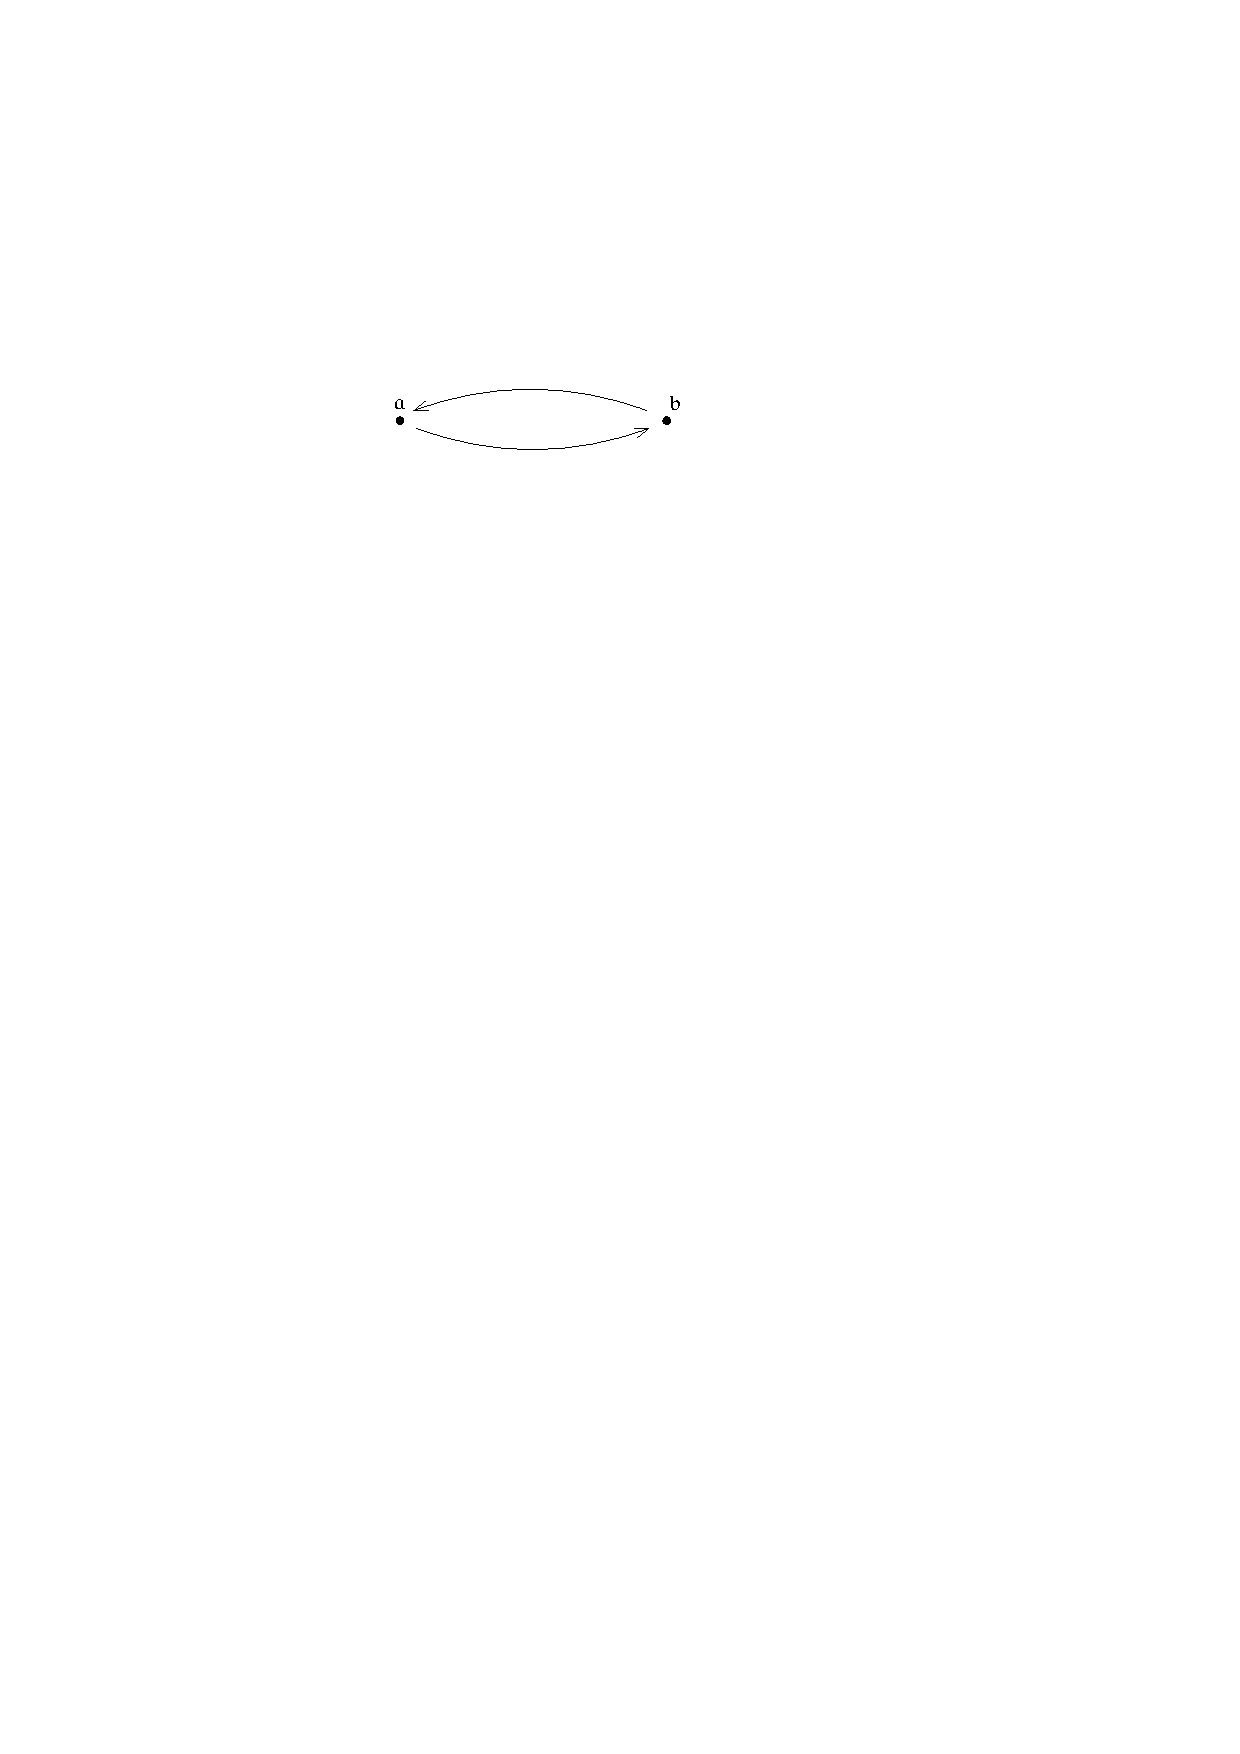
\includegraphics{../Figures/cat_2.pdf}
\]
Note that whenever we draw a category, we omit the identity morphisms. They are implied, and serve only to clutter the diagram. We also omit implied compositions of morphisms. In this case, because the identity morphisms are the only elements of $C(a,a)$ and $C(b,b)$, it must be that the two drawn morphisms compose to the identity morphisms.


We observe $\zeta$ defined on $C$ is
\[\begin{bmatrix}1 & 1 \\ 1 & 1 \end{bmatrix}.\]
This is not an invertible matrix. So this simple category does not admit M\"obius inversion.
\end{examp} 

\section{Euler-Leinster Characteristic of a Category}
We are now ready to construct central definition of this section: the Euler-Leinster characteristic (or just Euler characteristic) of a category. The entire construction can be found in \cite{Lein1, Lein2, Lein4}. 

\begin{defn}\label{def_weighting}
A \emph{weighting} on a category $\Aa$ is a function $\omega$ on $\obj(\Aa)$ such that for all $a \in \Aa$,
\[
\sum_{b \in C}|C(a,b)|\omega(b) = 1,
\]
or, equivalently, if
\[
\sum_{b \in C}\zeta(a,b)\omega(b) = 1.
\]
\end{defn}

One of the first questions we ask when we see this definition is how we can write find valid weightings. Luckily, this definition looks familiar. We have a value we know (1) expressed as the sum of function we are seeking ($\omega$). So we can use M\"obius inversion! The situation is slightly more complicated, because we don't know for sure that $\zeta$ is invertible. We formalize that:

\begin{lemma}
\label{mobius_is_weighting}
If $C$ has M\"obius inversion, then the weighting $\omega_\mu$ defined by $\omega_\mu(a) = \sum_b \mu(a,b)$ is a weighting on $C$.
\end{lemma}
\begin{proof} For all $a \in C$,
\begin{align*}
\sum_b \zeta(a,b)\omega_\mu(b) &= \sum_b\left( \zeta(a,b)\sum_c \mu(b,c)\right)\\
&=\sum_b\sum_c\zeta(a,b)\mu(b,c)\\
&=\sum_c\left(\sum_b\zeta(a,b)\mu(b,c)\right)\\
&=\sum_c \delta(a,c)\\
&=1.
\end{align*}
\end{proof}

Note that even if $C$ does not admit M\"obius inversion, it might admit a weighting. For example, the category in example \ref{2_pt} admits the weighting $\omega(a) = \omega(b) = 0.5$, even though it does not admit M\"obius inversion.

This is important. It provides a way in which we can write down weightings on metric spaces, since the similarity matrix $\zeta$ is invertible in many cases. We will investigate exactly which cases when we discuss positive semidefinite matrices.

The following definition is due to \cite{Lein1}.
\begin{defn}\label{cat_euler}
Let $\omega$ be a weighting on a finite category $A$. Then the \emph{Euler-Leinster characteristic}, or just the \emph{Euler characteristic}, of $A$, denoted by $\chi(A)$, is defined by
\[
\chi(A) = \sum_{a \in A} \omega(a)
\]
\end{defn}
Note that even if a category admits several weightings, they all lead to the same Euler characteristic by a simple sum rearrangement argument. Together with \ref{mobius_is_weighting}, this implies the following:
\begin{cor}\label{euler_mu}
If a finite category $A$ has a M\"obius inversion $\mu$, then
\[\chi(A) = \sum_{a \subseteq A} \sum_{b \subseteq A} \mu(a, b).
\]
\end{cor}
%TODO: Think of category w/ no euler char
\section{Simplicial Complexes}
Calling a new construction an Euler characteristic needs some intuitive justification. We will introduce a structure called a \textit{simplicial complex} to show that calling this value an Euler characteristic is reasonable. 

The most elementary form of an Euler characteristic is the version defined on polyhedrons: Vertices minus edges plus faces. As a result, it is common to think of the Euler characteristic as a value defined on geometric objects. A simplicial complex is a generalization of a polyhedron into higher dimensions. We use this construction because it has a natural notion of an Euler characteristic, which is consistent with the common one, and yet also is easily connected with categories. We start with the definition:

\begin{defn}
Let $V$ be a set. A \emph{simplicial complex} $\sigma$ over $V$ is a set of finite, non-empty subsets of $V$, called \emph{simplices} or \emph{cells}, such that, if $\alpha \in \sigma$ and $\emptyset \neq \beta \subset \alpha$, then $\beta \in \sigma$.
\end{defn}

Put another way, a simplicial complex over $V$  is a set of subsets of $V$ which is closed under taking subsets, with the exception of the empty subset. 

If a set in a simplicial complex $\sigma$ has $k$ elements, we call it a \emph{$k-1$-simplex} or a \emph{$k-1$-cell}. We think of 0-cells as vertices, 1-cells as edges, 2-cells as faces, etc. This will become much clearer with some examples.
\begin{examp}
Let $V=\{a,b\}, \sigma_2 = \{\{a\},\{b\}, \{a,b\}\}$. Then $\sigma_2$ is a simplicial complex over $V$. We visualize $\sigma_2$ as follows:
\[
\begin{tikzpicture}[auto, node distance = 3cm, main node/.style={dot}]

\node[label = above:{$\{a\}$}, circle, draw, fill=black,
                        inner sep=0pt, minimum width=4pt](1) at (0,0) {};
\node[label = above:{$\{b\}$}, circle, draw, fill=black,
                        inner sep=0pt, minimum width=4pt](2) at (3,0) {};

\draw[-latex] (1) -- (2) node[midway, above = 3pt] {$\{a,b\}$};

\end{tikzpicture}\]
Because $\{a\} \subseteq \{a,b\}$, the vertex $\{a\}$ is an endpoint of the line $\{a,b\}$. Because $\sigma_2$ is closed under taking subsets, as all simplicial complexes must be, the line has both its endpoints.
\end{examp}
Going forward, when writing down simplicial complexes, we will not explicitly write down the set $V$ - it will implicitly be the set of all elements used in the simplicies. We will also omit the braces around the subsets to reduce clutter. So we would write $\sigma_2 = \{a,b,ab\}$.

We saw in the previous example why it is that lines always have both their endpoints in the geometric representation of a simplicial complex. For the same reason, faces have all three edges. But the converse is not necessarily true - the outline of a triangle, for example, might exists without the triangle being filled.
\begin{examp}
Let $\sigma = \{a, b, c, d, ab, ac, bc, bd, cd, abc\}$. Then we draw $\sigma$ as follows:
\[
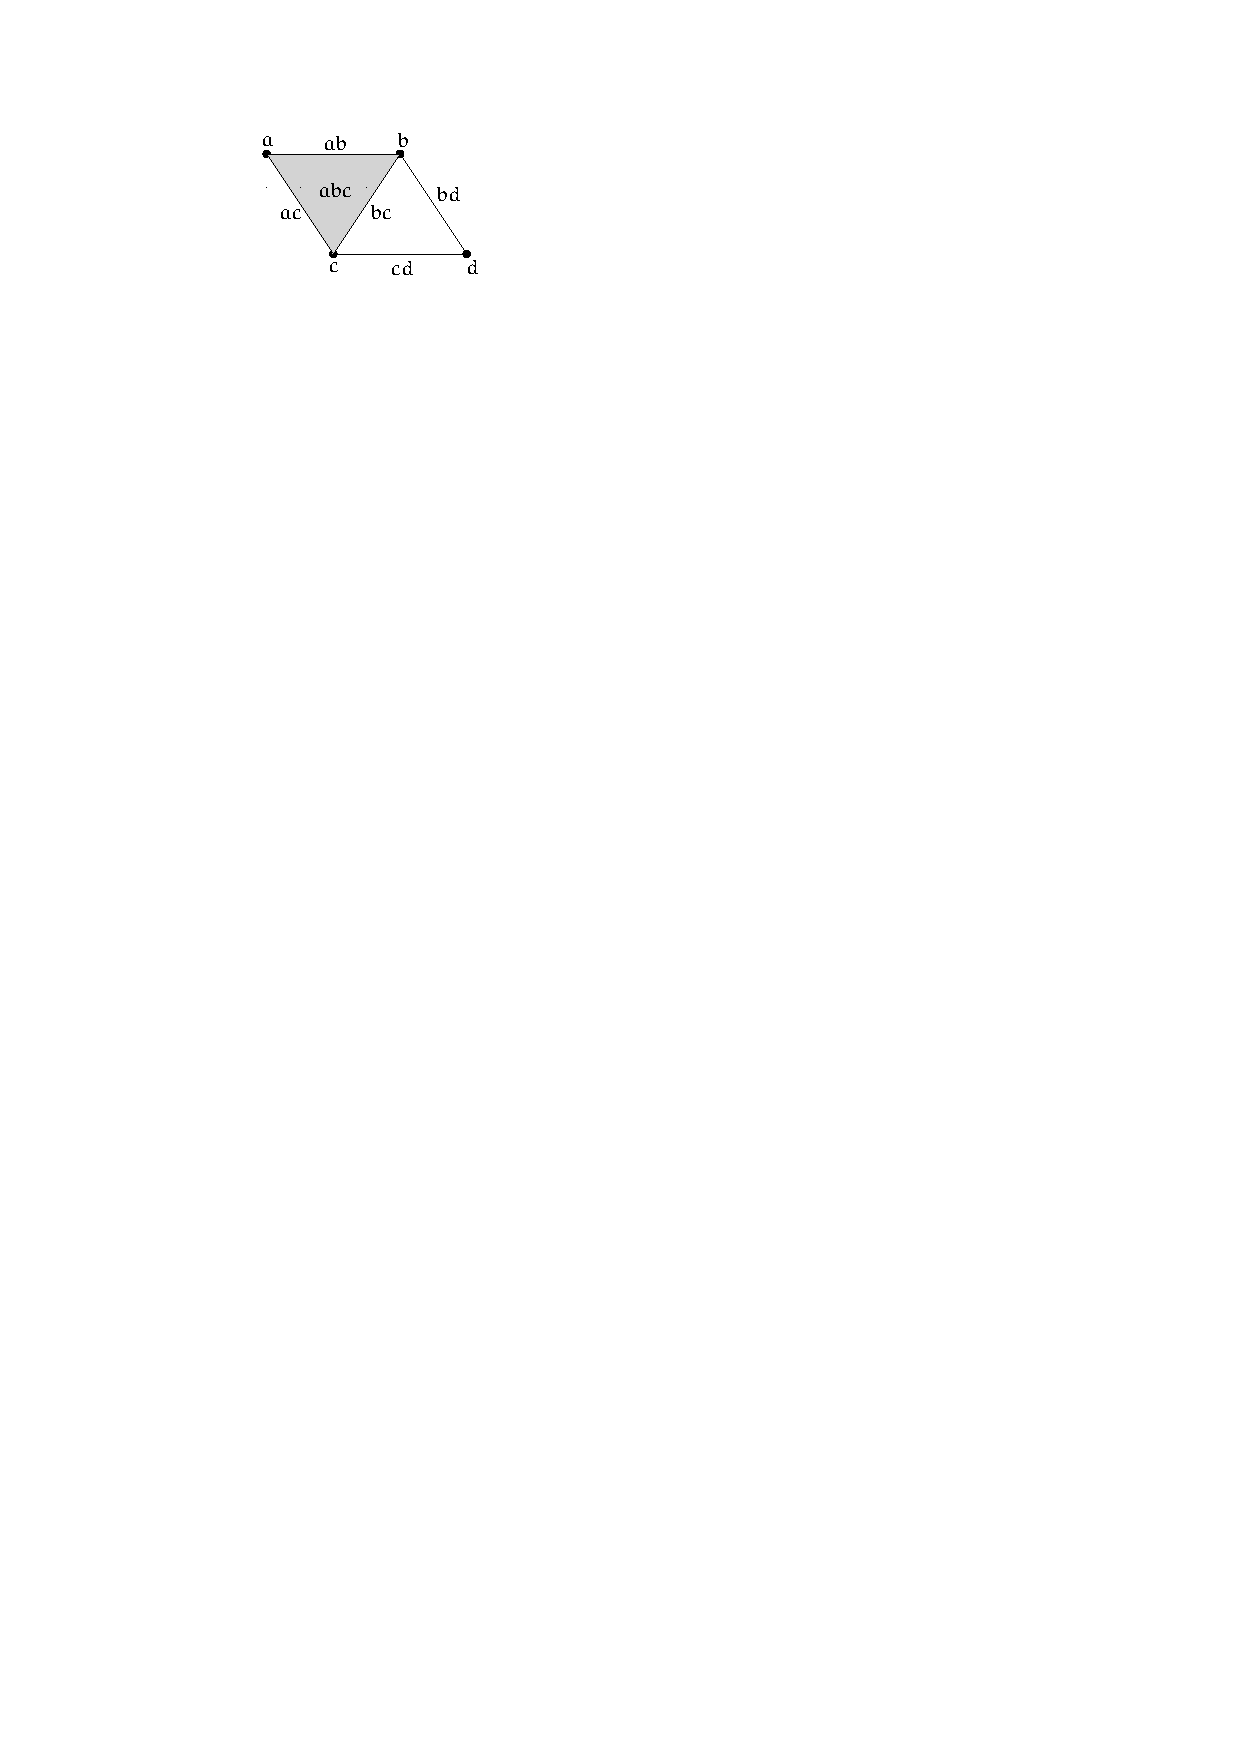
\includegraphics[scale = 1.3]{../Figures/simp_1.pdf}
\]
\end{examp}
As these examples illustrate, a $k$-simplex, or a simplex with $k+1$ elements, is considered to be a $k$-dimensional feature.

The goal of this construction was to justify our definition of the Euler characteristic of a category. To do that, we need to define the Euler characteristic of a simplicial complex.
\begin{defn}
Let $\sigma$ be a simplicial complex. Then the \emph{Euler characteristic} of $\sigma$, denoted by $\chi(\sigma)$, is equal to
\[
\sum_{\tau \in \sigma}(-1)^{|\tau|}.
\]
\end{defn}
Note that this is a distinct (although related) definition to \ref{cat_euler}, yet we use $\chi$ for both. Which we mean will be determined by what kind of object we are applying $\chi$ to. 

This definition is consistent with the definition of the Euler characteristic of a polyhedron: If the largest cells of a simplicial complex are 2-cells, or two-dimensional faces, then the definitions are identical. 

It turns out that there is a straightforward way of converting a simplicial complex into a category. We will find that the Euler-Leinster characteristic of the resulting category will be the same as the Euler characteristic of the simplicial complex. 
\begin{defn}
Let $\sigma$ be a simplicial complex. Then the \emph{category generated by $\sigma$}, or $\cat(\sigma)$, is the category whose objects are the cells of $\sigma$. If $\alpha$ and $\beta$ are cells of $\sigma$, then $|(\alpha, \beta)| = 1$ if $\alpha \subseteq \beta$ and 0 else.
\end{defn}
Note that a simplicial complex can be converted into a poset, where the cells are ordered by inclusion. Recall that we also defined $\cat(X)$ for a poset $X$ in \ref{cat_poset}. If $\sigma$ is a simplicial complex, and $X$ is the corresponding poset, then $\cat(\sigma) = \cat(X)$.

The notation for $\cat(\sigma)$ is a little tricky. If $\sigma$ is a simplicial complex, and $\alpha \in \sigma$ is a simplex, then we write $\cat(\alpha)$ to denote the object in $\cat(\sigma)$ corresponding with the simplex $\alpha \in \sigma$. We consider an example.
\begin{examp}
Let $\sigma = \{a, b, ab\}$. Then we can draw $\sigma, \cat(\sigma)$:
\[
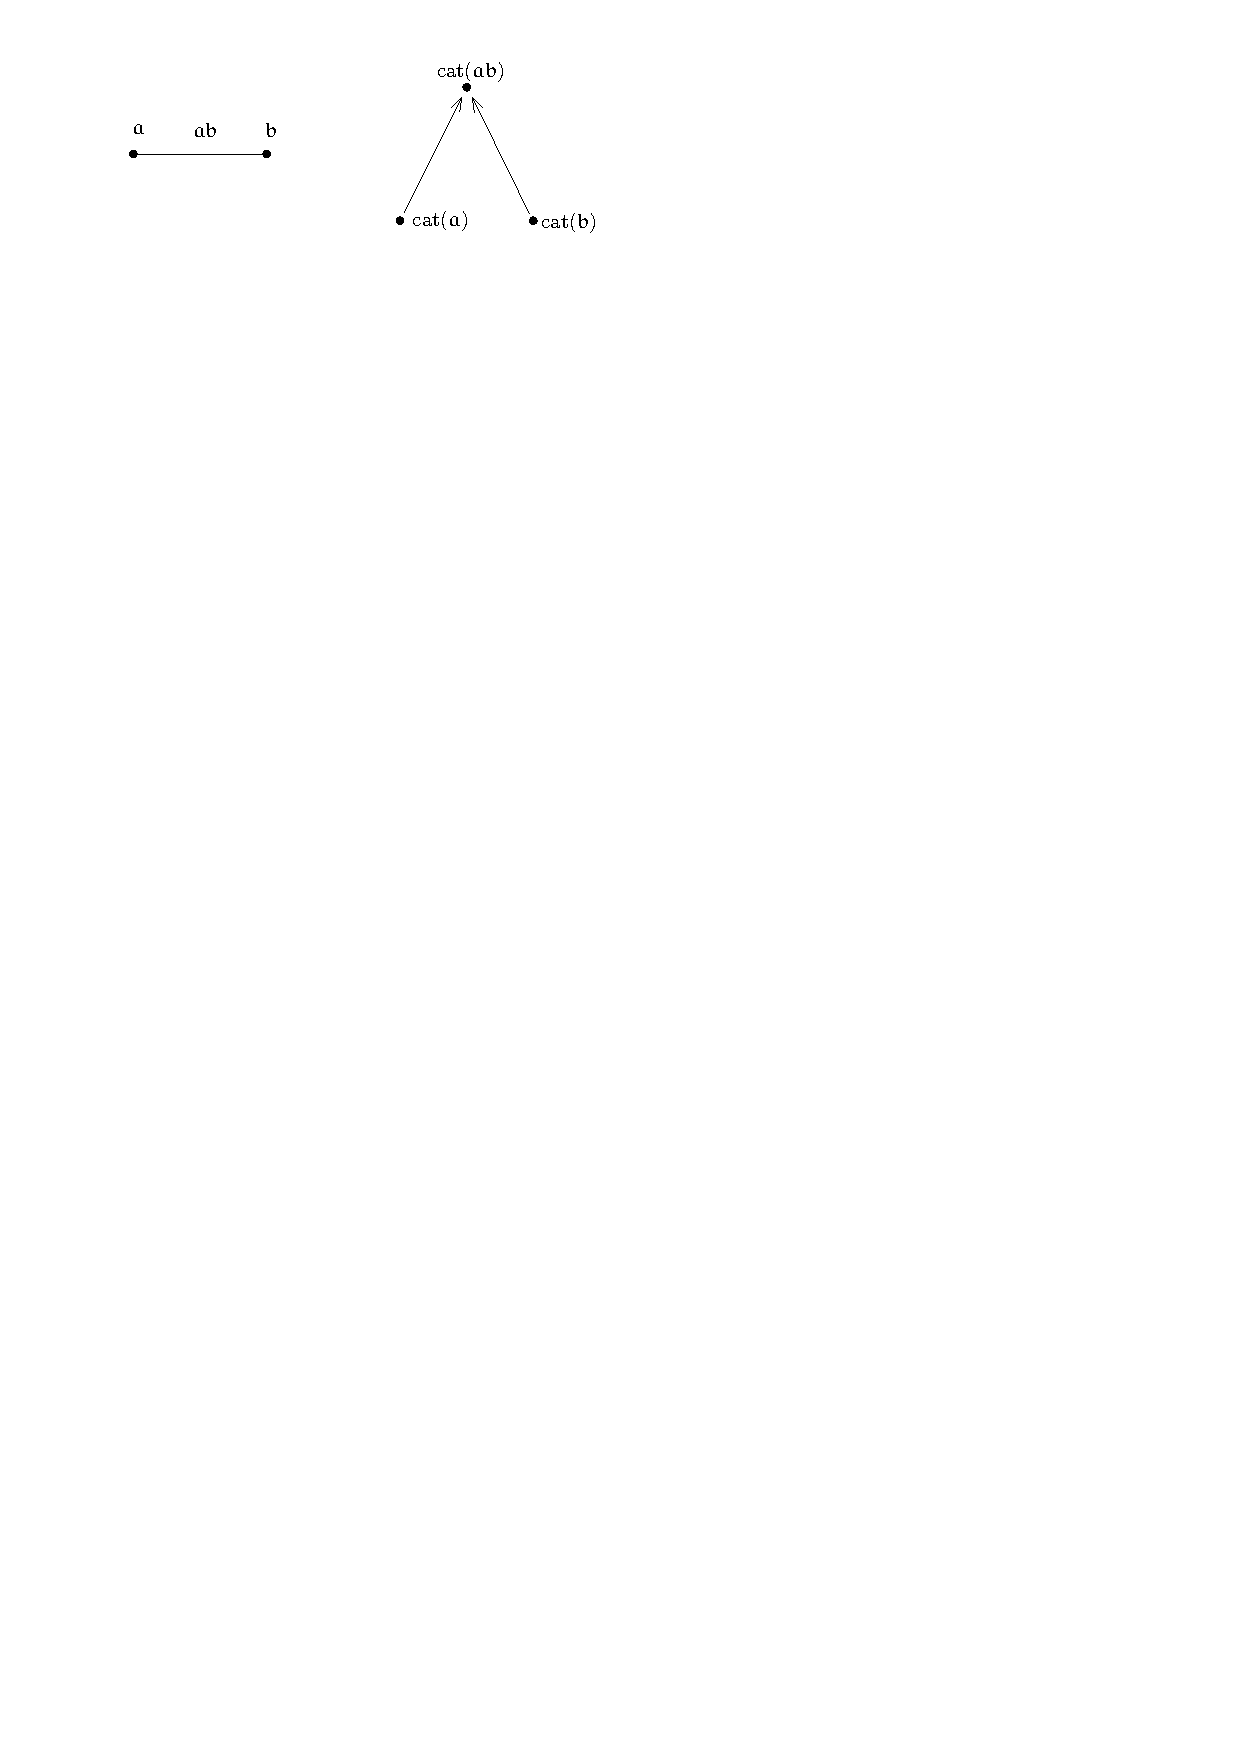
\includegraphics{../Figures/simp_cat.pdf}
\]
\end{examp}
Recall that we omit identity morphisms when drawing a category.

To prove that this operation preserves the Euler characteristic, we start with two lemmas about $\mu$, the M\"obius function on a category. First, recall that categories do not necessarily admit M\"obius inversion. So $\mu$, a priori, might not exist on a given category. However, the following lemma will rule this possibility out in the case of the category generated by a simplicial complex.
\begin{lemma}\label{mu_exists}
Let $\sigma$ be a simplicial complex. Then $\cat(\sigma)$ admits M\"obius inversion.
\end{lemma}
\begin{proof}
Totally order the simplices of $\sigma$ respecting the partial order of number of elements (so if $\alpha, \beta \in \sigma$ and $|\alpha| < |\beta|$, then $\alpha < \beta$ in the total order). Write down the matrix $\zeta$ with the rows and columns in that order. Then $\zeta$ will be upper triangular, so it will be invertible. So $\mu = \zeta^{-1}$ exists.
\end{proof}
Now that we know $\mu$ exists, we can inductively determine its value, similarly to how we have done so in previous sections with M\"obius functions on partially ordered sets.
\begin{lemma}
\label{mu_lemma}
Suppose $\sigma$ is a simplicial complex, and $\alpha \subseteq \beta$ are simplices in $\sigma$. Let $\mu$ denote the M\"obius function on $\cat(\sigma)$. Then $\mu(\cat(\alpha), \cat(\beta)) =(-1)^{|\beta - \alpha|} = (-1)^{|\alpha|} (-1)^{|\beta|}$ (note that $|\alpha|$ simply denotes the size of $\alpha$ as a set).
\end{lemma}
\begin{proof}
We use induction. Base case: $\alpha = \beta$, and $\mu(\alpha, \beta)=1$.

For the inductive step, suppose that if $|\beta-\alpha| \leq k$, the result is true.

Suppose that $|\beta - \alpha| = k+1$. We know by \ref{cat_mob} that, because $\alpha \neq \beta$,
 \begin{align*}
\sum_{\alpha \subseteq \sigma \subseteq \beta} \mu(\alpha, \sigma)&= 0\\
\mu(\alpha, \beta) &=  - \sum_{\alpha \subseteq \sigma \subset \beta} \mu(\alpha, \sigma)\\
&= - \sum_{\gamma \subset (\beta - \alpha)} \mu(\alpha, \gamma \cup \alpha) 
\end{align*}
Note that the above unions are always disjoint. So, by the inductive hypothesis, we can rewrite it:
\begin{align*}
\mu(\alpha, \beta) &= - \sum_{\gamma \subset (\beta - \alpha)'} (-1)^{|\gamma \cup \alpha - \alpha|} \\ %& \text{inductive hypothesis}\\
&= - \sum_{\gamma \subset (\beta - \alpha)'} (-1)^{|\gamma|}\\ % &\text{by disjointness}\\
\end{align*}
We can add and subtract $(-1)^{|\beta - \alpha|}$ and apply a binomial identity to finish the proof:
\begin{align*}
\mu(\alpha, \beta) &= - \sum_{\gamma \subseteq (\beta - \alpha)} (-1)^{|\gamma|} + (-1)^{|\beta - \alpha|} \\ 
&= (-1)^{|\beta - \alpha|} -  \sum_{i = 0}^{|\beta - \alpha|}(-1)^i{|\beta- \alpha| \choose i}\\ 
&= (-1)^{|\beta - \alpha|} \\ 
\end{align*}
\end{proof}
We are now ready to prove that the two definitions of the Euler characteristic coincide.
\begin{thm}
\label{consistentEuler}
Let $\sigma$ be a simplicial complex. Then 
\[
\chi(\cat(\sigma)) = \chi(\sigma).
\]

\end{thm}
\begin{proof}
Recall that by \ref{cat_euler}, 
\[
\chi(\cat(\sigma)) = \sum_{\gamma \in \sigma} \sum_{\alpha \in \sigma} \mu(\cat(\alpha), \cat(\gamma)).
\]
We know that if $\alpha \not \subseteq \gamma, \mu(\alpha, \gamma) = 0$. So
\[
\chi(\cat(\sigma)) = \sum_{\gamma \in \sigma} \sum_{\emptyset \neq \alpha \subseteq \gamma}\mu(\cat(\alpha), \cat(\gamma)).
\]
So we have
\begin{align*}
\chi(\cat(\sigma)) &= \sum_{\gamma \in \sigma} \sum_{\emptyset \neq \alpha \subseteq \gamma}\mu(\cat(\alpha), \cat(\gamma))\\
&= \sum_{\gamma \in \sigma} \sum_{\emptyset \neq \alpha \subseteq \gamma}(-1)^{|\gamma| - |\alpha|} &\text{by \ref{mu_lemma}}\\
&= \sum_{\gamma \in \sigma}(-1)^{|\gamma|} \sum_{i = 1}^{|\gamma|} (-1)^i{|\gamma| \choose i}\\
&= \sum_{\gamma \in \sigma} (-1)^{|\gamma|} \\
&= \chi(\sigma)
\end{align*}
\end{proof}
The fact that $\chi(\cat(\sigma)) = \chi(\sigma)$ is comforting. It justifies calling using $\chi$ in \ref{cat_euler}, and calling this construction a type of Euler characteristic.

\section{Euler-Leinster Characteristic Examples}


\end{chapter}
\begin{chapter}{Metric Space Magnitude}\label{chap_magnitude}
\section{Motivation: Hierarchical Clustering}
A common task in data analysis is clustering. Given a set of data points, it is often desirable to decide how many ``groups'' those data points fall into. Of course, there is usually no clear-cut definition of which points are in groups and which are not. 

The most straightforward way to cluster points is based on some notion of distance between them. If we assign a distance to each pair of points, then we can cluster points which are close together. But there is often no clear threshold for which points are and aren't close enough together to be in the same cluster. It all depends on the scale of structure we are looking for. One common technique for avoiding choosing a scale is what is called \emph{hierarchical clustering}. 

The idea of hierarchical clustering is that instead of choosing a scale, we capture the data's structure at a variety of scales:

\[
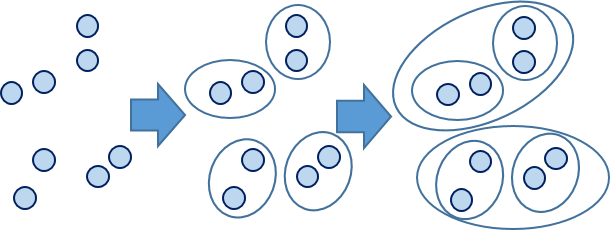
\includegraphics[width = 0.4\paperwidth] {../Figures/multiscale_structure.png}
\]

We can see that here that as we ``zoom out'', the structure of this data changes. First the data has first eight clusters of one point each, then four clusters of two points, and finally two clusters of four points. If we kept going, we would end up with a single cluster containing all of the points.

There are many methods of hierarchal clustering. In the above example, explicit clusters are formed by grouping points which are near each other. We will explore an alternate method of clustering, which does not actually construct clusters, but instead estimates the number of clusters using a real, rather than integer, value. We will use a generalization of the Euler-Leinster characteristic from chapter \ref{chap_euler}. We start by building some important definitions.

A metric space is a space with a notion of distance between pairs of points. 
\begin{defn}
A \textit{metric space} $(M,d)$ is a set $M$ together with a function  $d:M \times M \rightarrow \Rr$ (the \emph{metric}), such that the following are satisfied for all $a,b,c \in M$:
\begin{itemize}
\item $d(a,b) \geq 0$, with equality $\iff a = b$;
\item $d(a,b) = d(b,a)$; and
\item $d(a,b) + d(b,c) \geq d(a,c)$.
\end{itemize}
We sometimes write just $M$ if the metric is unambiguous.
\end{defn}

In almost all forms of hierarchical clustering, we represent data as a metric space. Here, we will actually define a slightly different structure which will be quite similar to a metric space, and use that instead. However, it's useful to keep in mind this more fundamental definition of a set with distance.

In the next section, we expand the Euler-Leinster characteristic to a generalization of categories called \emph{enriched categories}. We will connect this back to data and metric spaces in subsequent sections.
\section{Enriched Categories}
In chapter \ref{chap_euler}, we defined a structure called a category. It turns out that this construction - which we will now call an \emph{ordinary} category - can be generalized further, to become an \emph{enriched} category. The idea is that we replace the sets of morphisms with objects from an ordinary category of a certain type, and adapt the definition of composition accordingly. 

%TODO: Fix Furthermore, the definitions and constructions we explore will be easy to apply directly to metric spaces. I point out that this construction is a type of category to justify dealing with them together with other categories in the next section. We will define the Euler characteristic of a category, and we will need to apply the definition to metric spaces by way of generalized metric spaces. This will make much more sense if we keep in mind that generalized metric spaces are categories.

In order to define the next construction, we need to define a notion of isomorphism between objects in a category.
\begin{defn}
Let $C$ be an ordinary category. Let $x,y \in C$ be two of $C$'s objects. Suppose that $f \in C(a,b), g \in C(b,a)$ are morphisms such that $g \circ f = 1_x, f \circ g = 1_y$. Then we say
\begin{itemize}
\item $f = g^{-1}, g = f^{-1}$
\item $f$ and $g$ are \emph{inverses} of each other
\item $f$ and $g$ are both \emph{isomorphisms}
\item $f \cong g$
\item $a$ and $b$ are \emph{isomorphic}.
\end{itemize}
\end{defn}

If two objects $a$ and $b$ are isomorphic, then for any morphism to or from either $a$ or $b$, we can use the isomorphisms to construct an ``equivalent'' map to or from the other object. As a result, $a$ and $b$ are equivalent in nearly every way. The next several definitions will replace requirements for - for example - associativity with requiring associativity up to isomorphism. This is common in category theory, and makes definitions more versatile, although it also makes them seem much more complicated at first. 

\begin{defn}\label{def_monoid}
A \emph{monoidal category} is an ordinary category $A$, together with
\begin{itemize}
\item A \emph{monoidal product} $\otimes : A \times A \rightarrow A$;
\item A \emph{unit object} $u \in A$;
\end{itemize}
such that
\begin{itemize}
\item For each ordered triple of objects $x,y,z \in A$, $(x \otimes y) \otimes z \cong x \otimes (y \otimes z)$
\item For each $x \in A$, $u \otimes x \cong x \cong x \otimes u$,
\item The function $\otimes$ is \emph{functorial}. This essentially means that if $x_1, x_2, y_1, y_2 \in M, f \in C(x_1, x_2), g \in C(y_1, y_2)$, then there exists a corresponding morphism in $C(x_1 \otimes y_1, x_2 \otimes y_2)$. We call that morphism $f \otimes g$, and require that it behave as we would expect (e.g. if $f,g$ are both isomorphisms, $f \otimes g$ also is).
\end{itemize} 
\end{defn}
There are a variety of commutation requirements which we are not considering in detail here. The property of being functorial is also more involved. For a full account, see \cite{Kelly1}.

We turn to several examples of monoidal categories.
\begin{examp}
The category $\catname{set}$ is the prototypical example of a monoidal category. In that case, the monoidal product $\otimes$ is the tensor product on sets (hence the notation $\otimes$ for the monoidal product), and $u = \{*\}$, some set with a single element.

Here, we can consider what the required isomorphisms look like. It's required that for any set $X \in \catname{set}, \{*\} \otimes X \cong X$. Elements of $\{*\} \otimes X$ are of the form $(*, x)$ for $x \in X$. Also recall that an isomorphism is an invertible morphism, and that in \catname{set}, morphisms are just maps. So, because $|X| = |\{*\} \otimes X|$, the two sets are isomorphic in \catname{set}. The associativity isomorphisms are similar.
\end{examp}
\begin{examp}\label{cat_real}
A monoidal category which will be very important here is $\Rr^{\geq 0}$, where there is exactly one morphism $f \in \Rr(a,b)$ if $a \geq b$. The monoidal product is addition, and the unit object is 0. The requirements are easily checked. We will refer to this category as $D$, because soon it will be used to represent distances.

In this case, there are no need for isomorphisms, because for any $a,b,c \in \Rr^{\geq 0}, (a + b) + c = a + (b + c)$, and $0 + a = a = a + 0$. A monoidal category like this, where all the associativity and identity isomorphisms are the identity, is called a \emph{strict} monoidal category. In fact, in $D$, no two distinct elements are isomorphic. 
\end{examp}
We are now ready to partially define an important generalization on ordinary categories. This definition is highly technical, and a full understanding of it is not necessary for this investigation. So we will not spend much time exploring examples or intuition beyond the specific applications we need.
\begin{defn}\label{en_cat}
Let $M$ be a monoidal category. Then a \emph{category enriched by $M$} consists of
\begin{itemize}
\item A set $C_0$ of objects;
\item For each $a,b \in C_0$, an \emph{object of morphisms} $C(a,b) \in M$;
\item For each $a,b,c \in C_0$, a \emph{composition morphism} $\circ_{abc}:  (C(b,c) \otimes  C(a,b)) \rightarrow  C(a,c)$;
\item For each $a \in C_0$, an \emph{identity element morphism} $i_a : u \rightarrow C(a,a)$, where $u$ is the unit object in $M$,
\end{itemize}
such that all the $i_1, \circ_{abc}$ commute appropriately.
\end{defn}
As with ordinary categories, we usually will omit the subscripts on the composition morphisms. They will be implied by context.
\begin{rmk}
For a full discussion of enriched categories, including a complete description of the commutation requirements, see \cite{Kelly1}. 
\end{rmk}

\section{Norms and the Euler-Leinster Characteristic}
The following constructions can be found in \cite{Lein4}.

We would like to generalize the weightings and Euler-Leinster characteristic from chapter \ref{chap_euler} so we can use them on enriched categories. Recall that in \ref{def_weighting}, we used the function $\zeta$ to require that for $\omega$ to be a weighting on a category $C$, for all $a \in C$,
\[
\sum_{b \in C}|C(a,b)|\omega(b) = 1.
\]

The problem is that given an enriched category over some monoidal category $M$, for a pair $a,b$, $C(a,b)$ is no longer a set but an element of $M$. So it is no longer possible to use the function $|\cdot|$ as defined on sets. Instead, we must define our own \emph{norm} function on $M$. We define this as follows:
\begin{defn}
Let $(M,\otimes)$ be a monoidal category. Then the function $| \cdot |: M \rightarrow \Rr$ is a \emph{norm} on $M$ if, for any $a,b\in M$, and if $u$ is the unit object of $M$, it satisfies
\[
|a \otimes b| = |a||b|,
\]
\[
|u| = 1.
\]
\end{defn}

The usual cardinality function on the monoidal category \catname{set} does satisfy these requirements - for any two finite sets $A,B, |A \otimes B| = |A||B|$, and $|\{*\}|=1$.

It's not clear why we require that the norm function be multiplicative. %TODO: If I get into products, discuss. Add more examples of norms

We can consider some examples of norms.
\begin{examp}\label{exp_norm}
Let $D$ be the monoidal category of non-negative real numbers defined in example \ref{cat_real}. Then, for all $t \in \Rr$, the function $|\cdot|:D \rightarrow \Rr$ defined by 
\[
|x| = e^{-tx}
\]
is a norm on $D$. We can see that it satisfies the requirements:
\[|0| = 1
\]
\[|x + y| = e^{-tx + ty} = |x||y|.
\]
We will explore this norm in detail shortly.
\end{examp}

Now that we know how to replace the norm function on sets, we can redefine the $\zeta$ function, M\"obius inversion, weightings, and the Euler-Leinster characteristic on enriched categories. We go through these definitions, and then we will explore their ramifications.
\begin{defn}
Let $C$ be a finite category enriched over a monoidal category $M$. Suppose that $|\cdot|$ is a norm on $M$. Then we define the similarity matrix $\zeta$ on $C$ by
\[
\zeta_{|\cdot|}(a,b) = |C(a,b)|.
\]
\end{defn}

\begin{defn}
Let $C$ be a finite category enriched over a monoidal category $M$. Let $|\cdot|$ be a norm on $M$, and let $\zeta_{|\cdot|}$ be the similarity matrix defined above. Then the M\"obius function on $C$, denoted $\mu_{|\cdot|}$, is defined by 
\[
\mu_{|\cdot|} = \zeta_{|\cdot|},
\]
if $\zeta$ is invertible. If $\mu$ exists, we say that $C$ admits M\"obius inversion.
\end{defn}

\begin{defn}
Let $C$ be a finite category enriched over a monoidal category $M$, with a specificed norm $|\cdot|$. Then $\omega$ is a \emph{weighting} on $C$ if, for all $a \in C$, 
\[
\sum_{b \in C}|C(a,b)|\omega(b) = 1,
\]
or, equivalently, if
\[
\sum_{b \in C}\zeta_{|\cdot|}(a,b)\omega(b) = 1.
\]
\end{defn}

\begin{defn}
Let $C$ be a finite category enriched over a monoidal category $M$, with a specified norm $|\cdot|$. Let $\omega$ be a weighting on $C$. Then the \emph{Euler-Leinster characteristic} of $C$, denoted $\chi_{|\cdot|}(C)$, is defined by
\[
\chi_{|\cdot|}(C) = \sum_{a \in c} \omega(a).
\]
\end{defn}
In the notation just introduced, we will sometimes omit the subscripts specifying the norm, if the norm is implied.
\begin{rmk}
When $C$ is an enriched category, $\chi(C)$ is sometimes called the \emph{magnitude} of $C$ (for example, in \cite{Lein4}). We reserve that terminology for a particular class of enriched categories which we will soon introduce, and continue to refer to the general construction as the Euler-Leinster characteristic or the Euler characteristic of $C$.
\end{rmk}
\begin{rmk}
As before, it is easy to show by rearranging terms that the value of $\chi_{|\cdot|}(C)$ is independent of the specific weighting chosen. However, it does depend on the norm we choose. This will become very important later.
\end{rmk}
%TODO: Examples of euler characteristics of non-metric space enriched categories

\section{Magnitude}
Recall that the motivation for this section was data clustering. So we would like to use the technology from the previous section to process data in the form of a metric space. We will use a particular enriched category for that purpose, called a \emph{generalized metric space}. This is a category enriched over a monoidal category whose objects are non-negative real numbers, allowing us to preserve a notion of distance. 
\begin{defn}\label{gen_met}
Let $D$ be the monoidal category of non-negative real numbers defined in example \ref{cat_real}. Let $C$ be a category enriched over $D$. Then we call $C$ a \emph{generalized metric space}.
\end{defn}
There is a lot of technology buried in that definition, and it can be difficult to untangle the definitions involved in enriched categories. Luckily, because of the simplicity of $D$, we can simplify the definition of a generalized metric space to one which does not depend on the definition of an enriched category.
\begin{thm}\label{direct_def}
A generalized metric space $C$ can be defined equivalently by the following:
\begin{itemize}
\item A collection $C_0$ of points (or objects); and
\item For each ordered pair $a,b \in C_0$, a non-negative real number $C(a,b)$
\end{itemize}
such that, for all $a,b \in C_0$,
\[C(a,a) = 0,
\]
\[\hspace{1cm} C(a,b) + C(b,c) \geq C(a,c).
\]
\end{thm}
\begin{proof}
We will start with the definition from \ref{gen_met}, and argue that it is equivalent to the above. As defined originally, a generalized metric space consists of a set of objects $C_0$, with a non-negative real number $C(a,b)$ between any ordered pair of elements $a,b \in C_0$. So what remains is to show that the composition requirements from \ref{en_cat} are equivalent to the conditions in \ref{direct_def}. 

Let $C$ be a generalized metric space as defined in \ref{gen_met}. Then \ref{en_cat} requires that there be a morphism $i_a:0 \rightarrow C(a,a)$ for any $a \in C$. This exists if and only if $C(a,a) \leq 0$, which is equivalent to saying that $C(a,a)=0$. So the existence of $i_a$ for all $a$ is equivalent to the first requirement above.

It is also required that for any $a,b,c \in C$, there is a map $\circ_{abc}: C(b,c) + C(a,b) \rightarrow C(a,c)$. This is equivalent to saying that $C(b,c) + C(a,b) \geq C(a,c)$, which is the second requirement. So the definitions are indeed identical.
\end{proof}

This makes it clear why we call this construction a generalized metric space. It is a metric space, but without the restriction that distinct points have nonzero distance, and without the requirement of symmetry. Relaxing these constraints allows us to cleanly express this as an enriched category.  

Generalized metric spaces are, of course, more general than ordinary metric spaces. So we can always express a metric space as a generalized metric space. This allows us to find the Euler-Leinster characteristic of a finite set of data points in a metric space. But first we must decide on the norm we will use on $D$, our monoidal category, and to do that, we take a step back and consider why we are doing this.

%TODO: Sports crowd analogy

So we would like a norm on $D$, the monoidal category of real numbers, which decreases as its argument get large. Recall that in example \ref{exp_norm}, we observed that the function $|x|=e^{-tx}$ is a norm on $D$. For any positive $t$, this is a decreasing function. In fact, we wills see that if we use this family of norms, we can view $t$ as a ``zooming'' parameter, which allows us to consider the data at different scales.

We have a special name for the Euler characteristic of a generalized metric space which results from this particular norm:
\begin{defn}
Let $M$ be a generalized metric space. Let $|\cdot|_t:D \rightarrow \Rr$ be defined by
\[
|x|_t = e^{-tx}.
\]
If it exists, let $\chi_t(M)$ be the Euler characteristic resulting from $|\cdot|$. Then $\chi_t(M)$ is called the \emph{$t$-magnitude} (or just \emph{magnitude} if $t=1$) of $M$, denoted $\magn_t(M)$ or just $\magn(M)$.
\end{defn}
%TODO: Small examples w/ graphs
\section{Product Spaces and Approximations}

Consider the following set of points $A$ in two-dimensional space:

\[
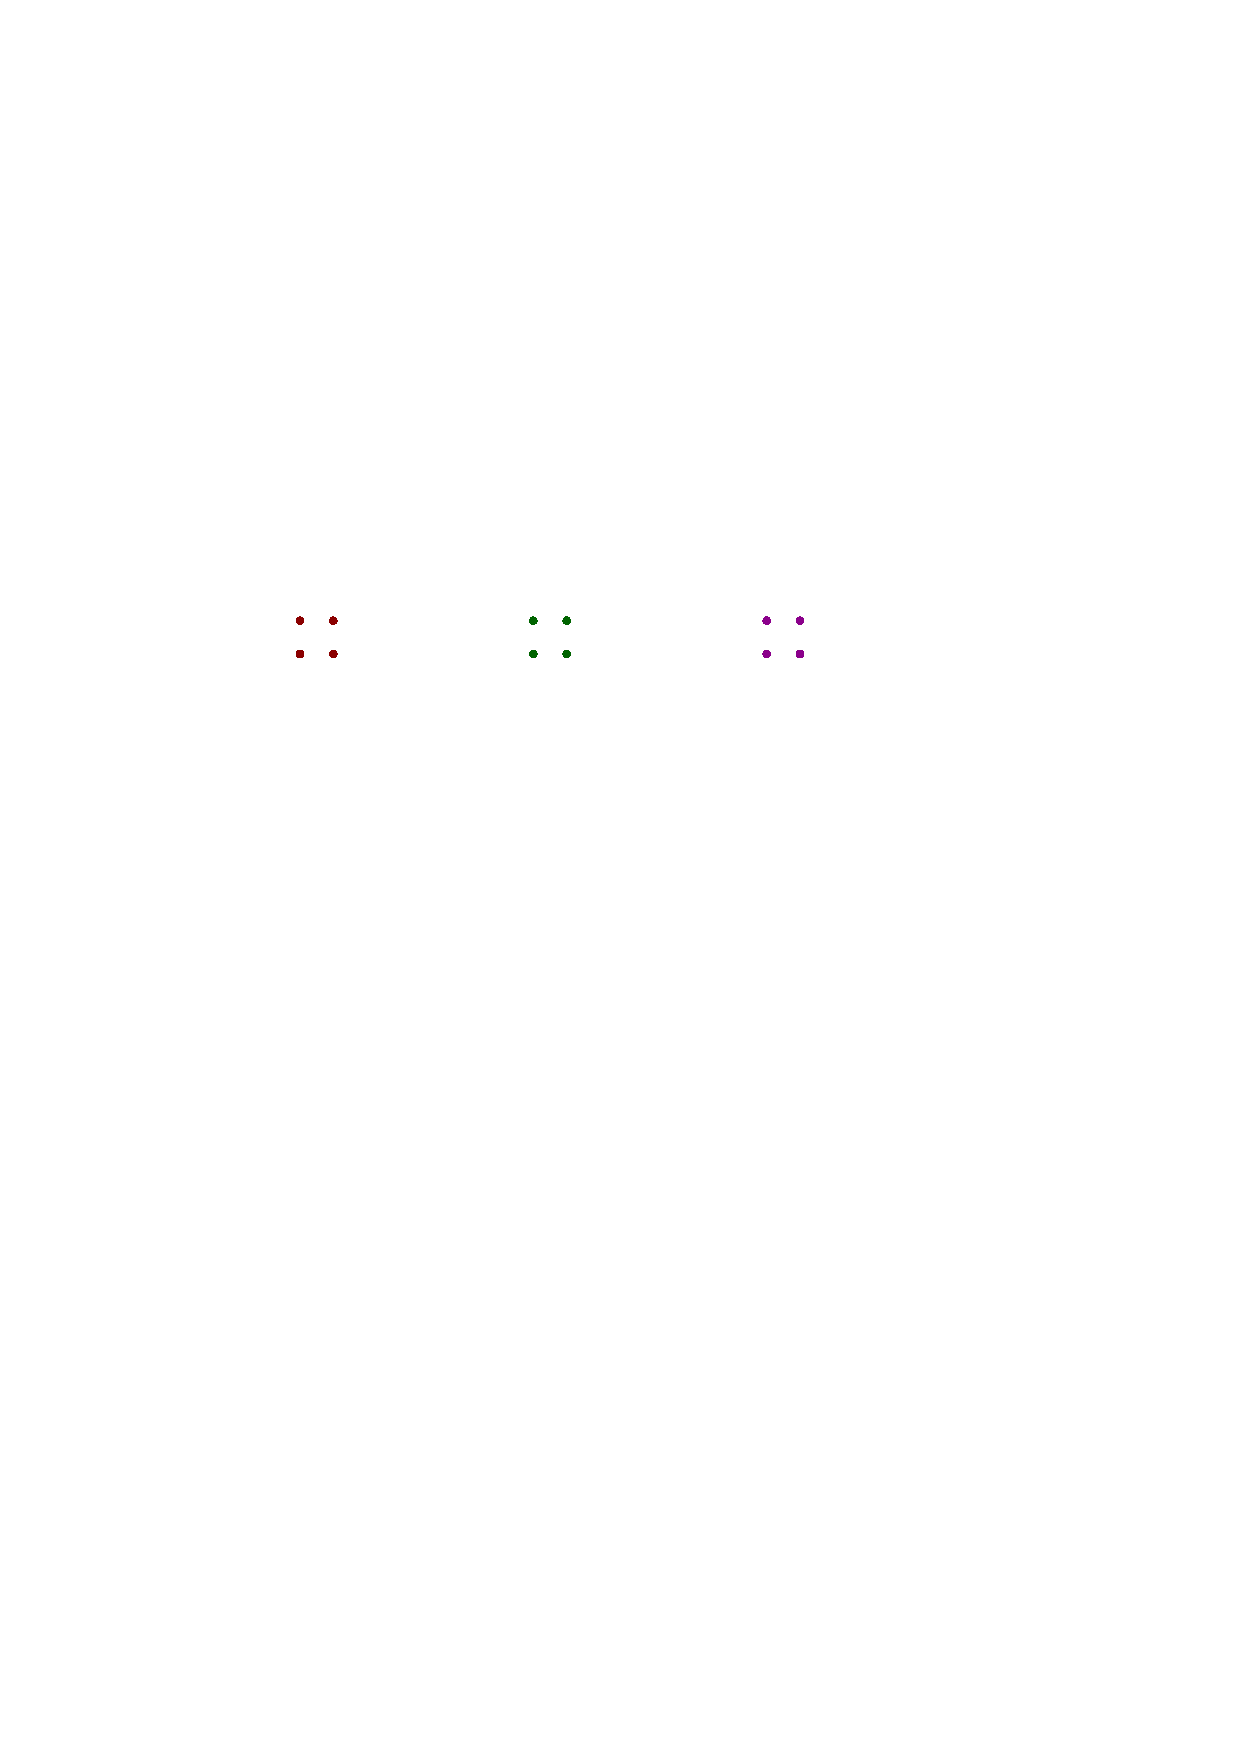
\includegraphics{../Figures/4x3.pdf}
\]

Let $M$ be this set:
\[
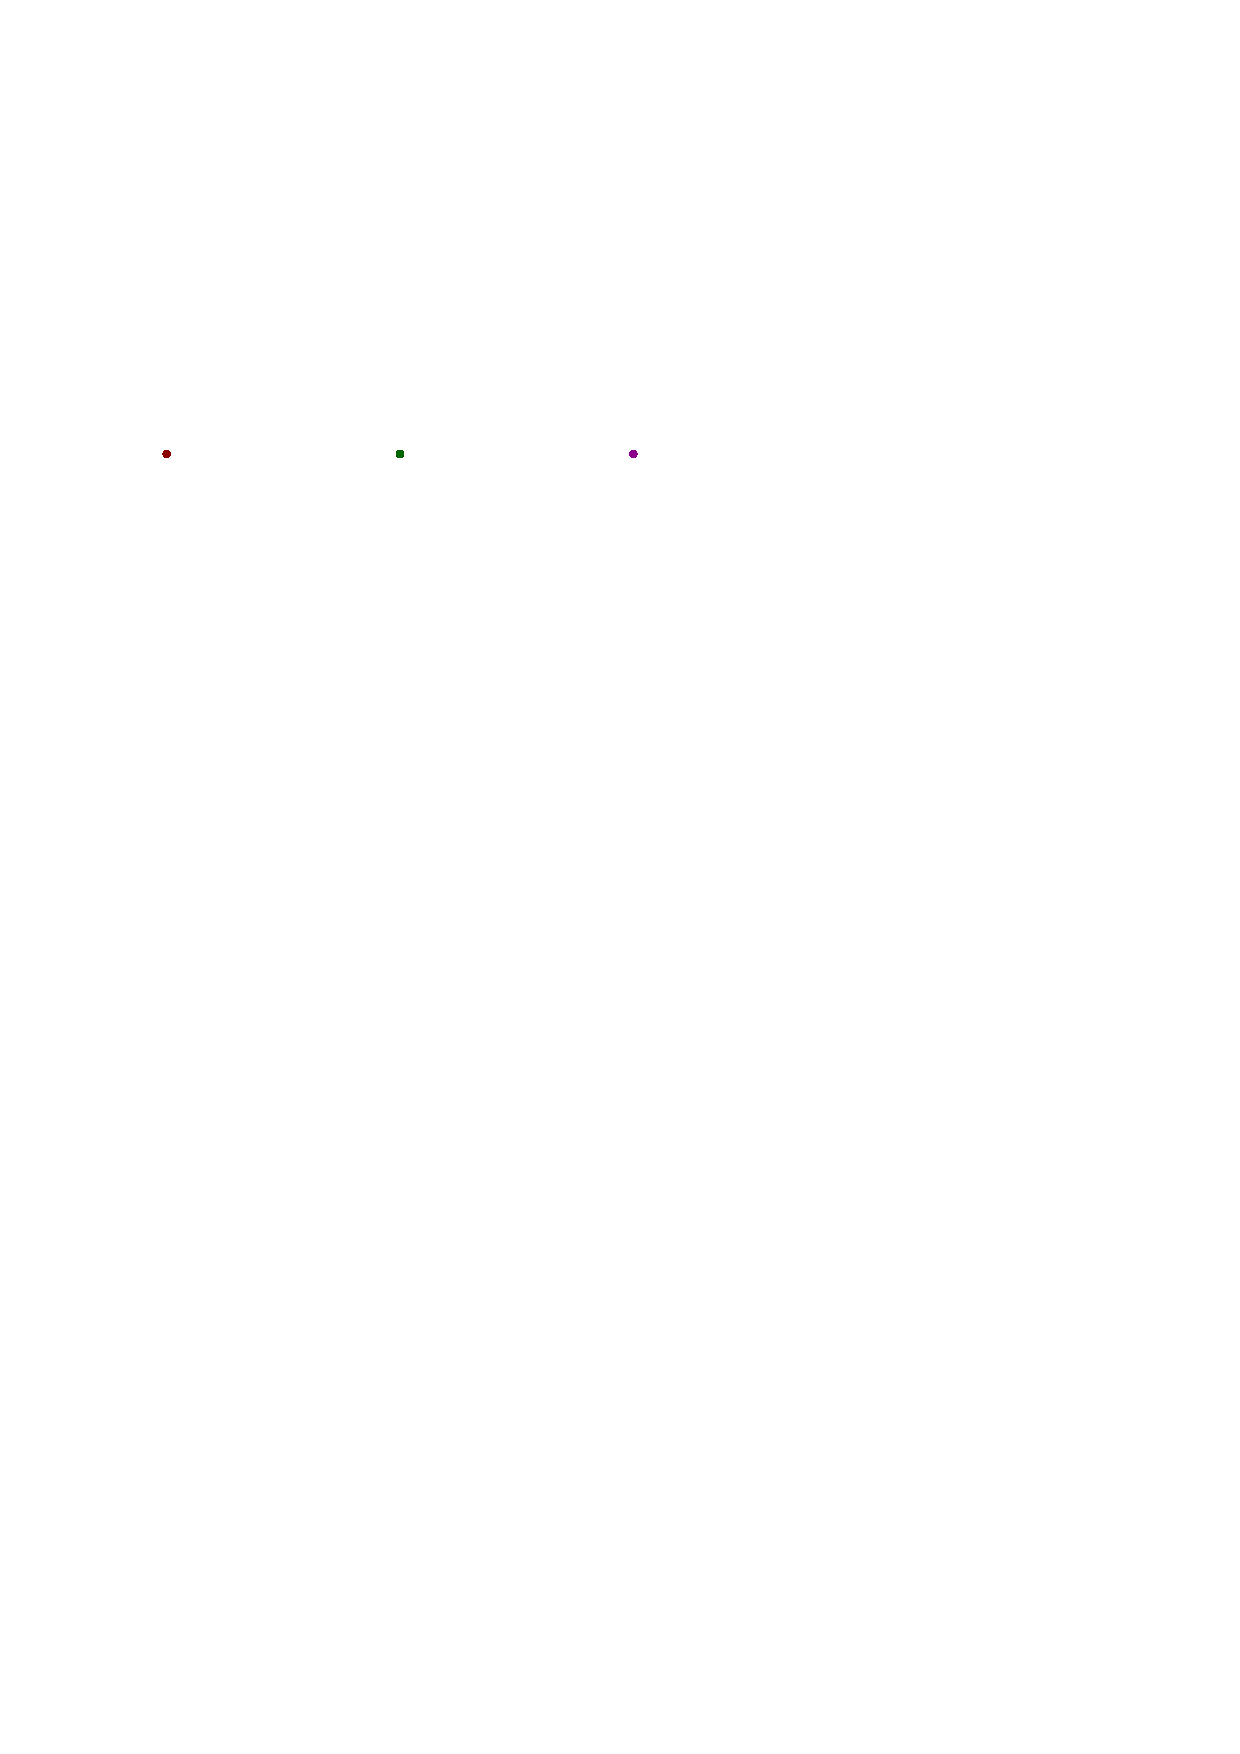
\includegraphics{../Figures/3.pdf}
\]

and $N$ this set:
\[
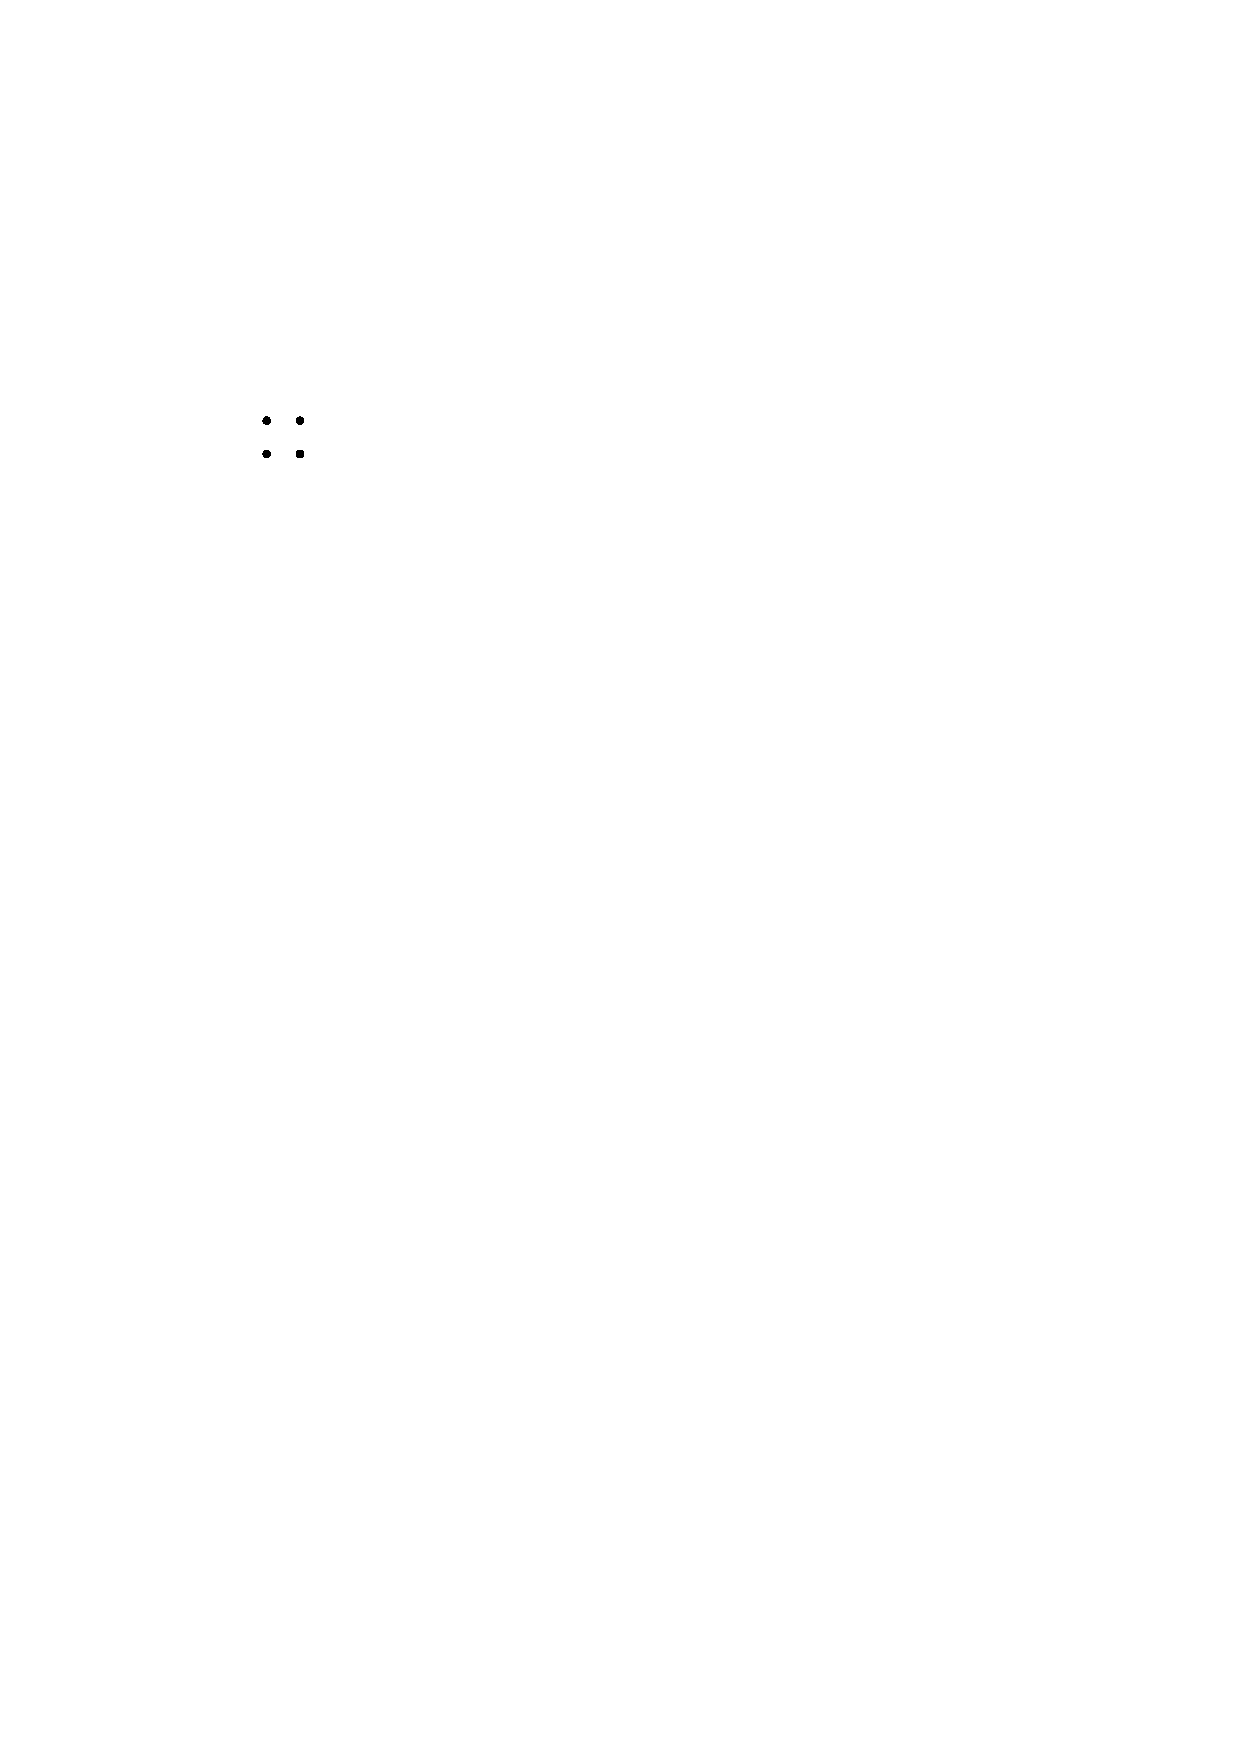
\includegraphics{../Figures/4.pdf}
\]

The set $A$ is what you would get if you replaced each point in $M$ with the set $N$. Suppose we choose a scale, and somehow count the number of clusters in $N$ and in $M$. 

If the scale is very small -- if we ``zoom in'' so that points must be very close together before they are considered to be in the same cluster -- then every point will be in its own cluster. So $N$ will have four clusters, $M$ three, and $A$ will have 12.

If we choose a middle scale, then it might be that the points in $N$ are clustered together, but $M$ remains discrete. Then $N$ has one cluster, $M$ has three, and $A$ has four, as each copy of $N$ forms a cluster.

Finally, if our scale is large enough that $M$ is grouped into a single cluster, all three sets of points will have a single cluster.

In all three cases, the number of clusters in $A$ is the product of the number of clusters in $M$ and in $N$. It appears that this remains the case as we change our scale. 

$A$ is an approximation of what is called a \emph{tensor product category}. In this section, we define the construction formally, and explore how the Euler-Leinster characteristic behaves when two categories are combined in this way. In particular, we would like for the magnitude of a product space to be the product of the magnitudes of the original spaces - this is how the number of clusters seems like it should behave when we look at examples like $A$ above.

Not all enriched categories can be used to construct product spaces. We first must define a restriction on the definition of a monoidal category.

\begin{defn}
Let $M$ be a monoidal category with monoidal product $\otimes$. Suppose that for all $a,b \in M, a \otimes b \cong b \otimes a$. Then $M$ is a \emph{symmetric monoidal category}.
\end{defn}

We add this restriction to allow us to prove the following lemma:

\begin{lemma}
Let $M$ be a symmetric monoidal category. Let $P,Q,R,S,T,U$ in $M$ be given. Suppose that we have morphisms
\begin{align*}
f&:(P \otimes Q) \rightarrow T\\
g&:(R \otimes S) \rightarrow U.
\end{align*}
Then, if $f \otimes g$ is the morphism required by the functoriality requirement of definition \ref{def_monoid}, we have
\[
(f \otimes g):(P \otimes Q) \otimes (R \otimes S) \rightarrow T \otimes U.
\]
\end{lemma}
\begin{proof}\label{prod_morph}
Using the symmetry of $\otimes$, we can rearrange:
\[
(P \otimes Q) \otimes (R \otimes S) \cong (P \otimes R) \otimes (Q \otimes S).
\]
Then definition \ref{def_monoid} tells us that the desired morphism exists.
\end{proof}
This extra requirement is necessary for the product of two enriched categories to exist. In particular, the composition maps do not necessarily exist if the monoidal category is not symmetric. We can now define that:

\begin{defn}
Let $A,B$ be categories both enriched over a symmetric monoidal category $M$. Fix a norm on $M$. Then the \emph{tensor product} of $A$ and $B$, denoted $A \times B$, is the category enriched over $M$ defined as follows:
\begin{itemize}
\item The set of objects, $(A \times B)_0$, is $\{(a,b):a \in A_0, b \in  B_0\}$
\item For $(a,b), (c,d) \in A_0, C((a,b), (c,d)) = C(a,b) \otimes C(c,d)$.
\item The unit object is $u_A \otimes u_B$, where $u_A, u_B$ are the units of $A,B$ respectively
\item The composition and identity morphisms are defined using Lemma \ref{prod_morph} (the details are not important for this discussion, but they are straightforward).
\end{itemize}
\begin{rmk}
The tensor product of two categories enriched over $M$ is indeed a category enriched over $M$. There are many requirements to check, and we do not go through all of them here.
\end{rmk}
\end{defn}

We consider some examples of simple product categories. Note that \catname{set} is a symmetric monoidal category, so ordinary categories are eligible to be used as factors of product categories. 
\begin{examp}
Let $A$ be the following category:
\[
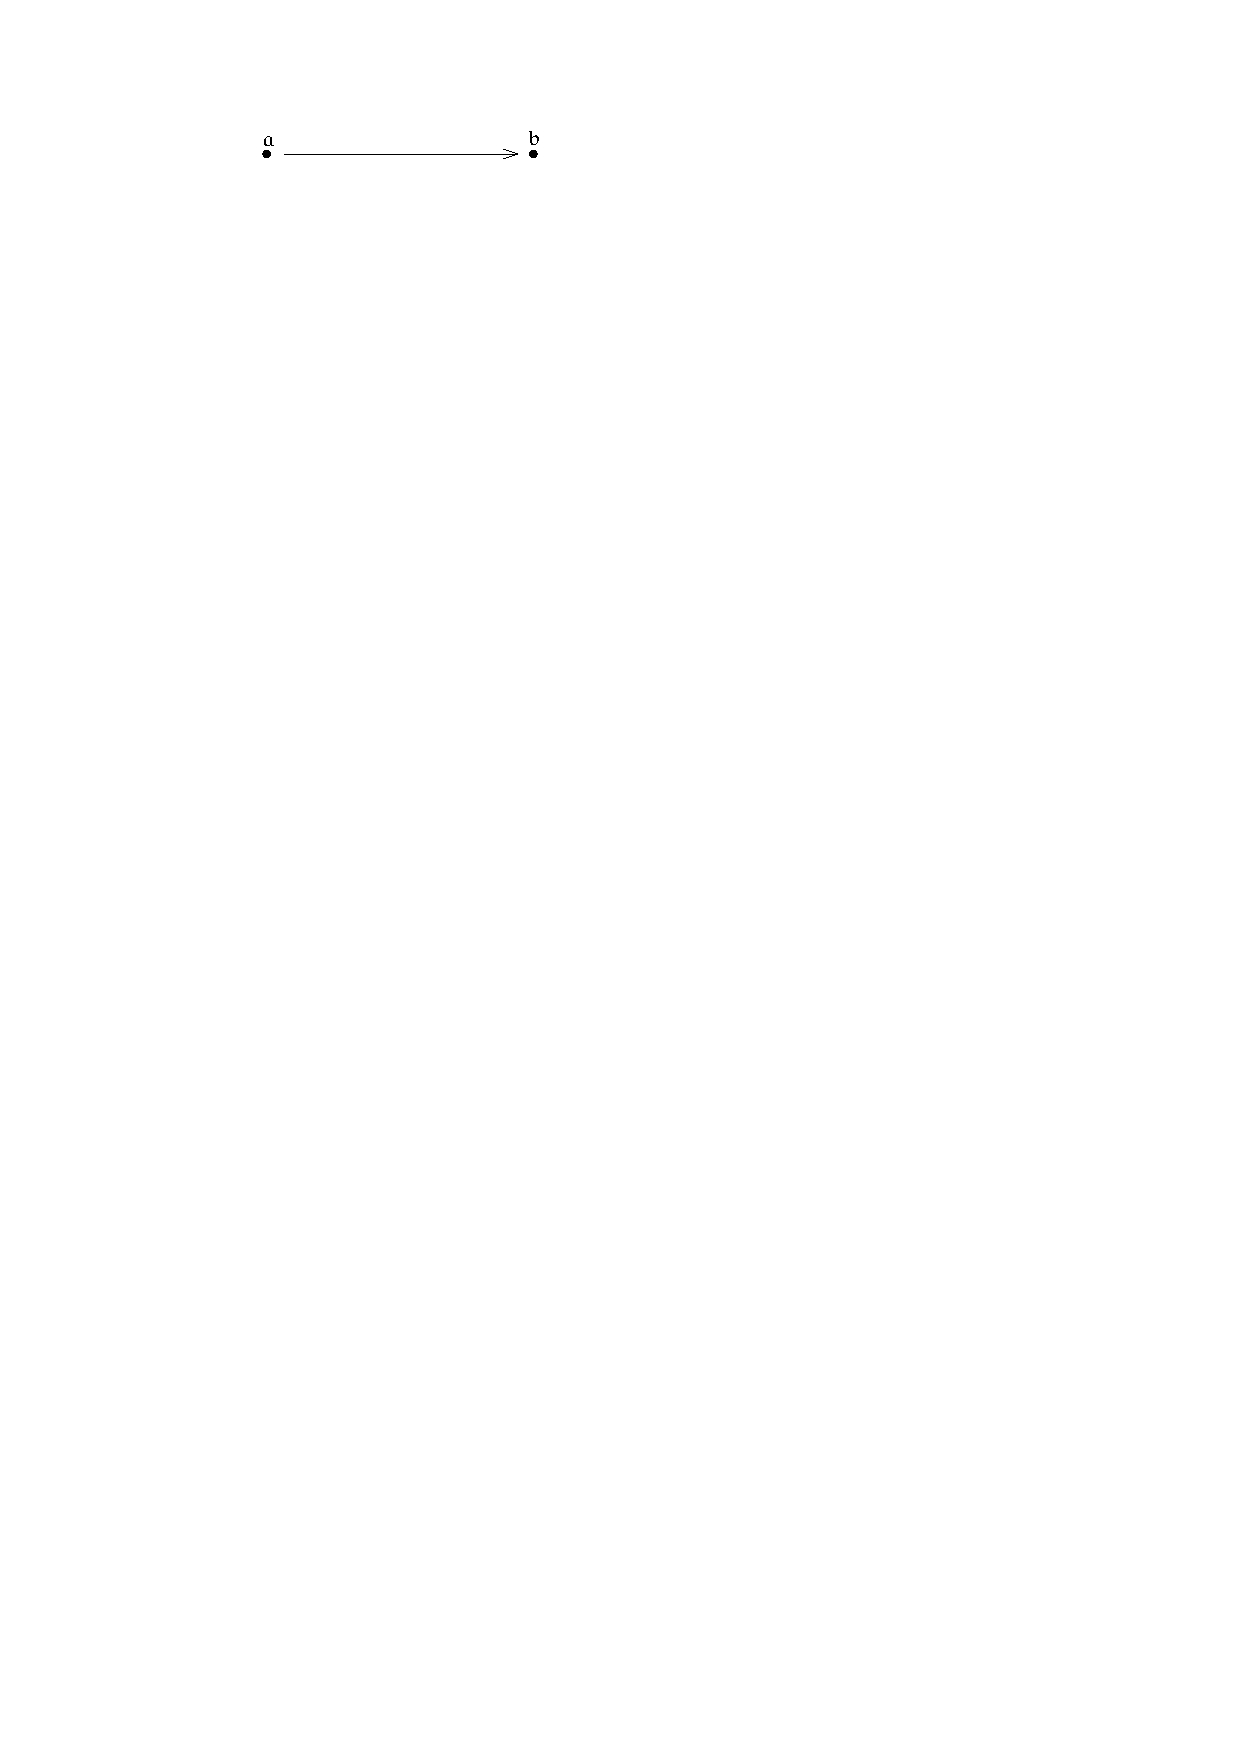
\includegraphics{../Figures/cat_2_directed.pdf}
\]
Recall that we omit the identity morphisms when we draw categories. So $A$ has two points and three morphisms. Then $A \times A$ looks like this:
\[
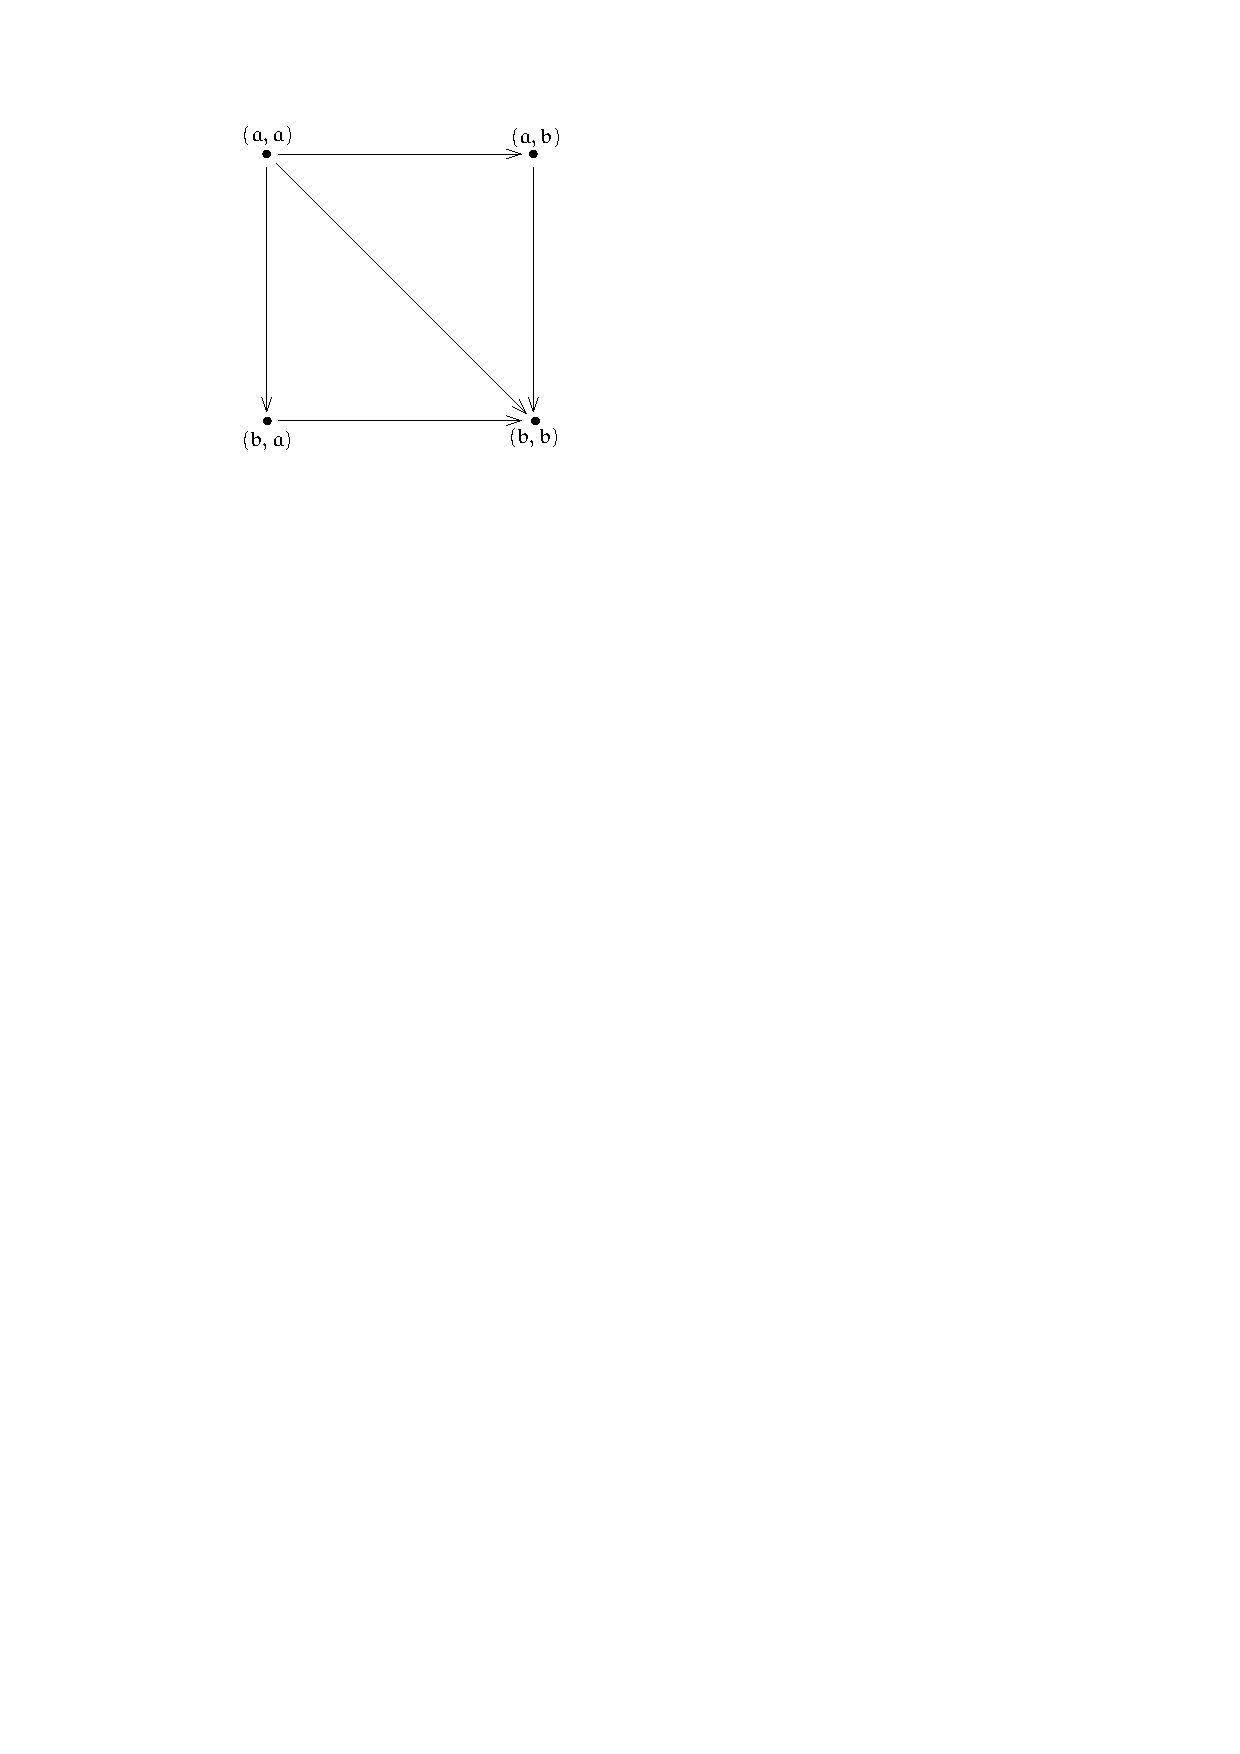
\includegraphics{../Figures/cat_2_prod.pdf}
\]
To see why, recall that the monoidal product on \catname{set} is the direct product. So consider, for example, $(a,a)$ and $(a,b)$. There is one morphism from $a$ to $a$ and one from $a$ to $b$. So the direct product of the hom-sets also has one element, which is why there is one arrow from $(a,a)$ to $(a,b)$. On the other hand, because there is no morphism $b$ to $a$, there is also no morphism from $(a,b)$ to $(a,a)$. 
\end{examp}
\begin{examp}\label{met_prod_ex}
We will be focusing on products of generalized metric spaces. So we consider an example of that. Let $A, B$ be the following:
\[
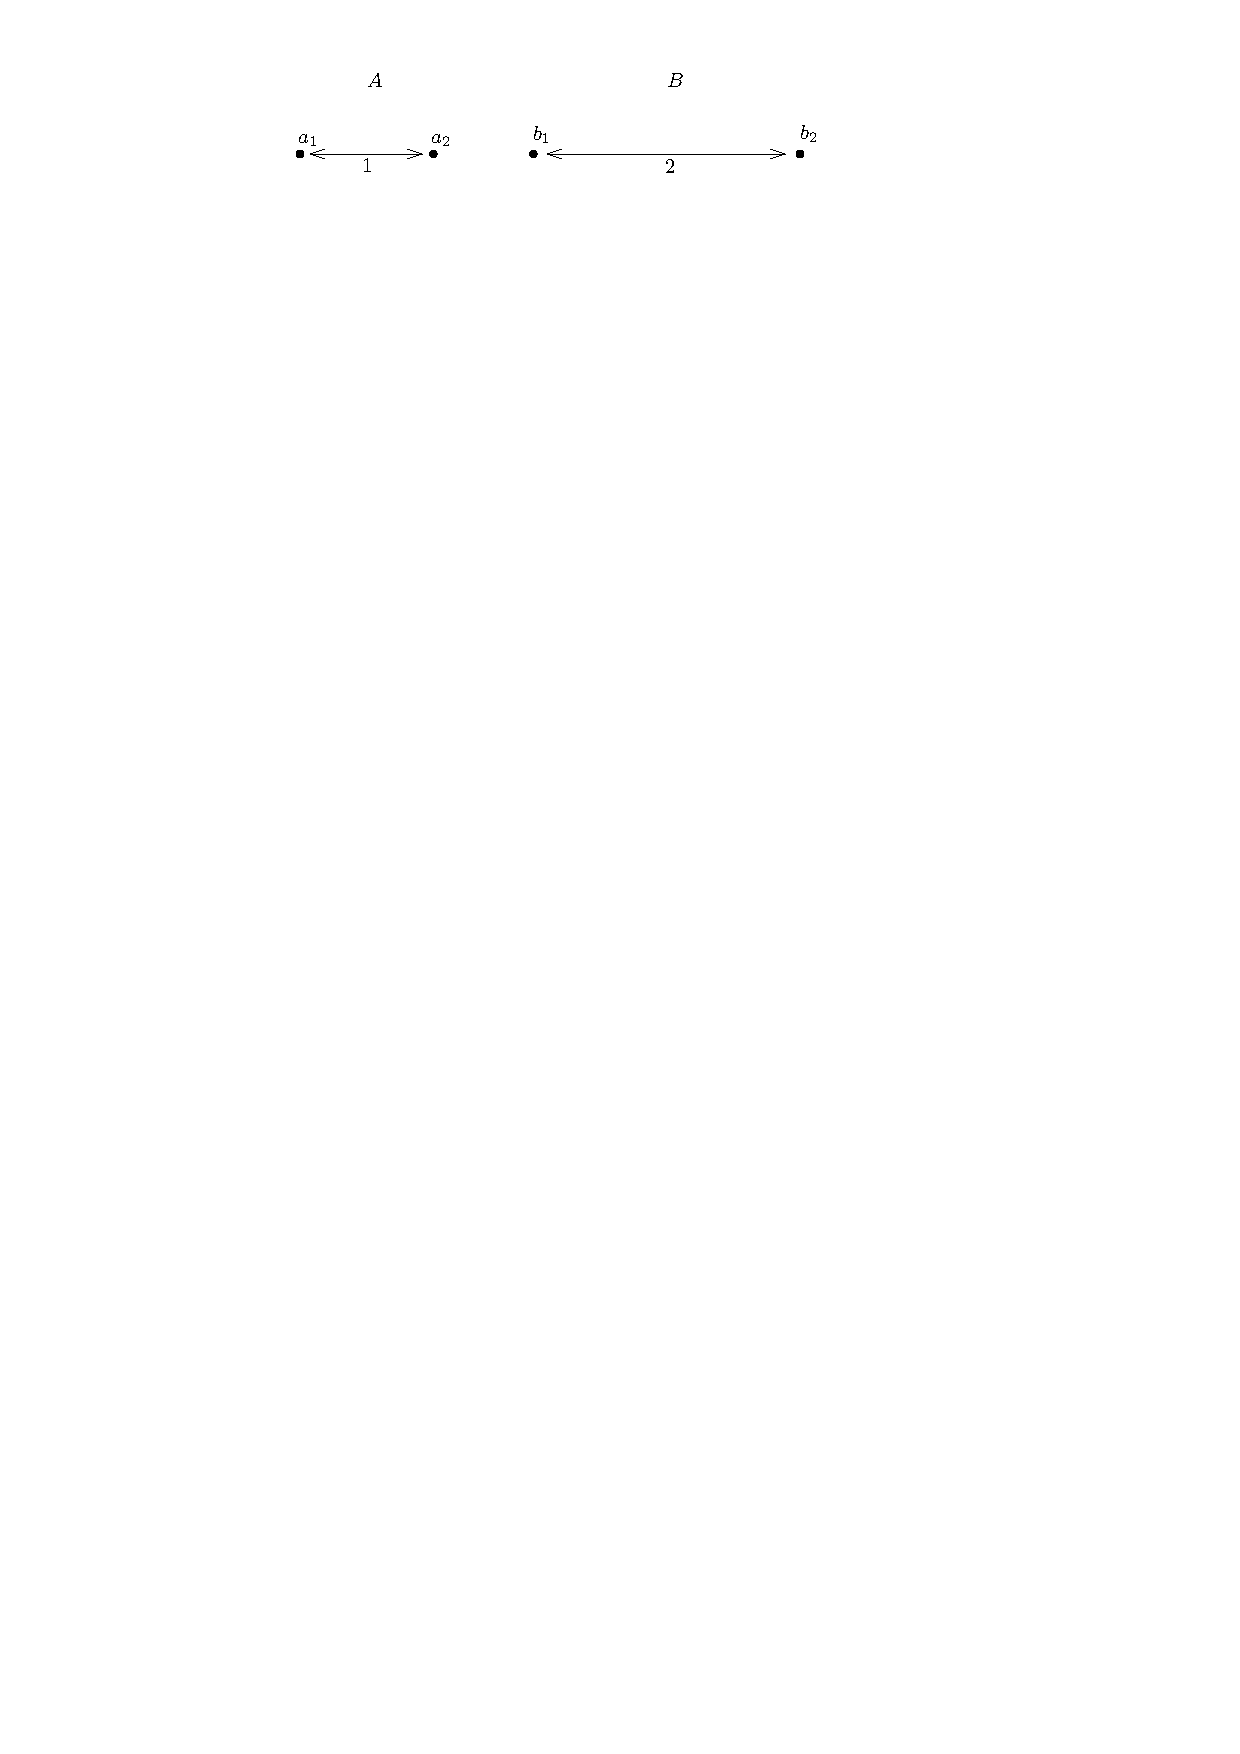
\includegraphics{../Figures/gen_met_small.pdf}
\]
So each space has two points, with $A(a_1, a_2) = 1, B(b_1, b_2) = 2$. Then the tensor product category $A \times B$ looks like this:
\[
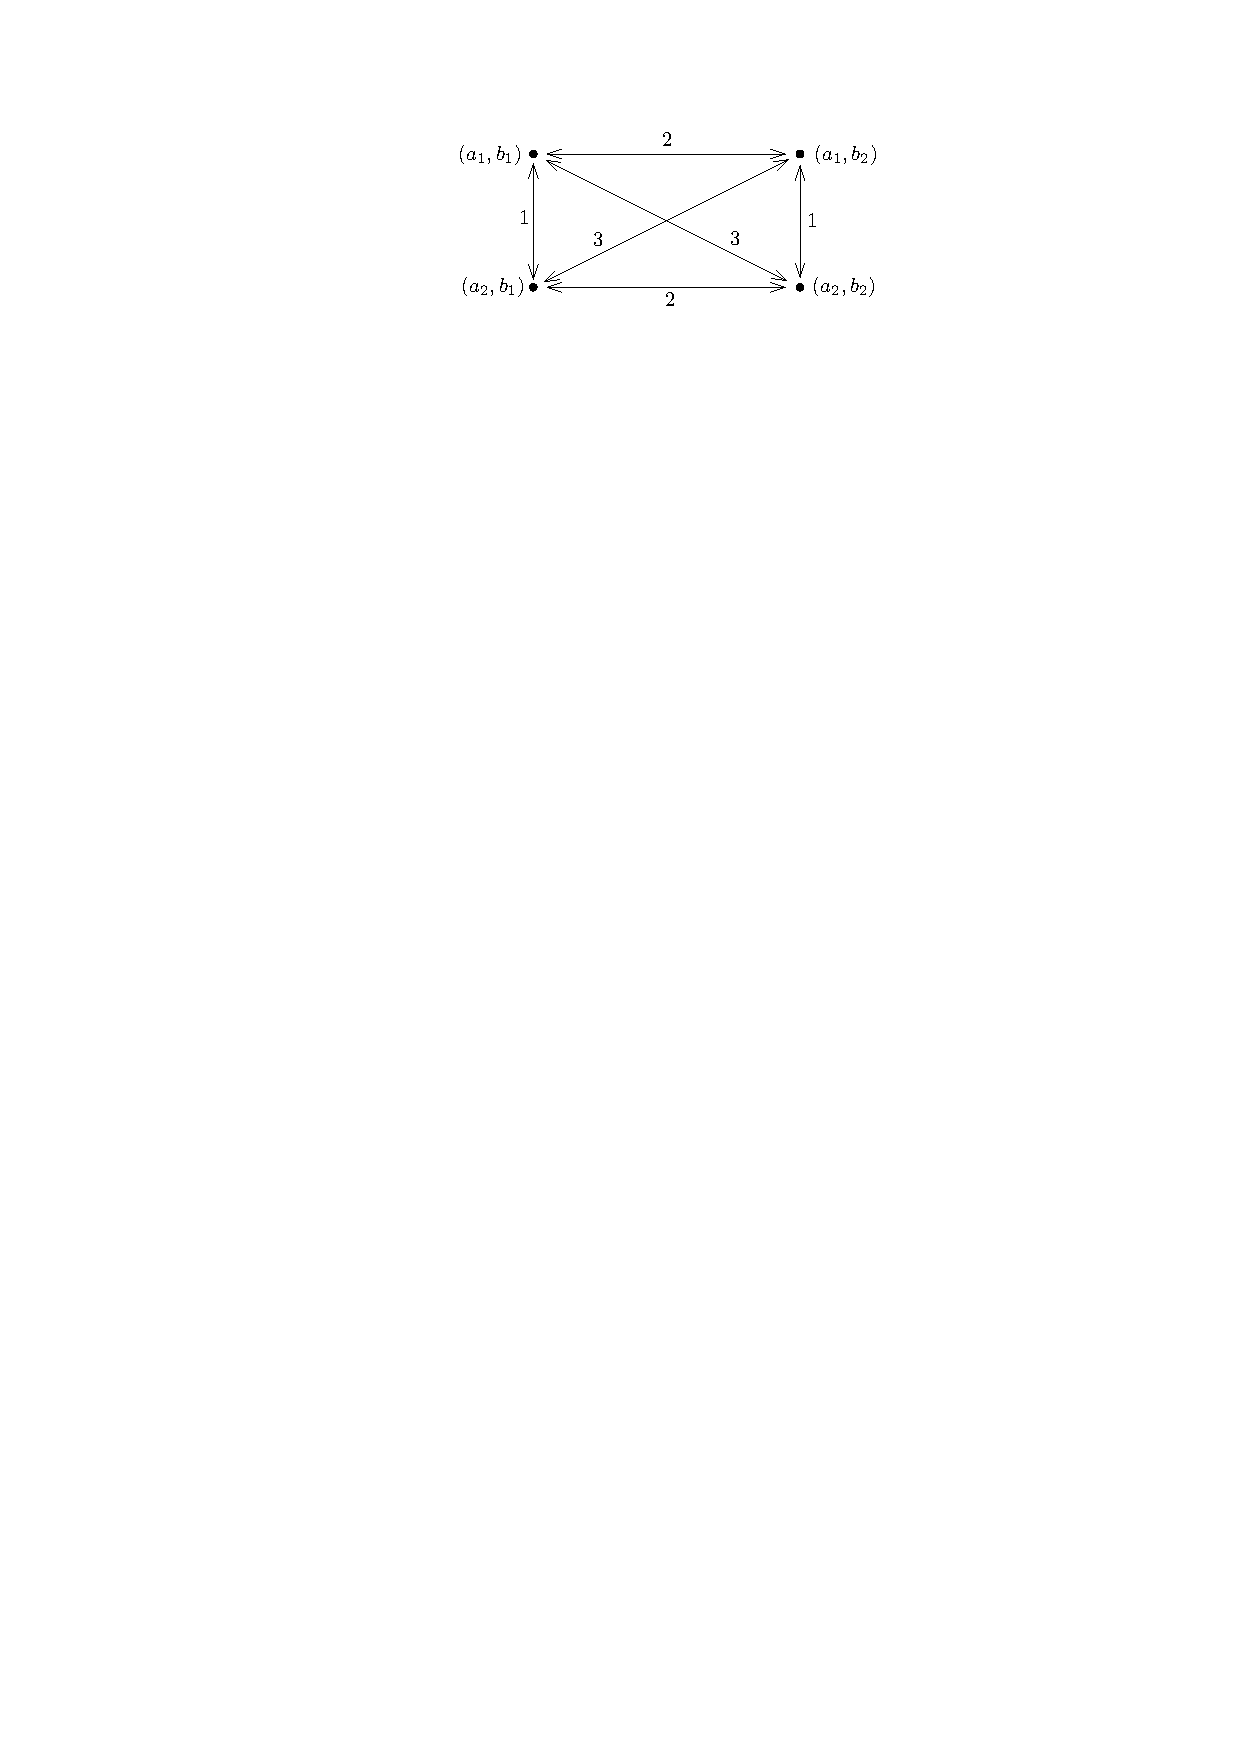
\includegraphics[width=.4\paperwidth]{../Figures/gen_met_small_prod}
\]
It is impossible to draw this product space to scale because of the way distances behave. 

We can observe the same behavior here as in the initial example. Suppose we used some clustering scheme where points within a threshold distance $t$ of each other were put into the same cluster. This is not how magnitude works, of course, but it is easier to visualize. Then we have three cases:
\begin{description}
\item[$t < 1$:] $A$ has two clusters, $B$ has two clusters, and $A \times B$ has four clusters.
\item[$1 \leq t < 2$:] $A$ has one cluster, $B$ has two clusters, and $A \times B$ has two clusters.
\item[$t \geq 2$:] $A, B$, and $A \times B$ each have just one cluster (note that $(a_1, b_2)$ and $(a_2, b_1)$ are in the same cluster in $A \times B$ even though their distance is 3, because both are in the same cluster as $(a_1, b_1)$).
\end{description}
So in all cases, the number of clusters in $A \times B$ is the product of the numbers of clusters in $A$ and $B$. We will see that this isn't a coincidence.
\end{examp}

Magnitude is obtained using $\zeta$, the similarity matrix. So we are interested in how the similarity matrix behaves under the tensor product. It turns out that the similarity matrix of a product category is obtained using the matrix \emph{Kronecker product}, not coincidentally (but confusingly) written using $\otimes$. 
\begin{defn}
Let $A$ be an $m \times n$ matrix and $B$ be a $q \times r$ matrix. Then the \emph{Kronecker product} of $A$ and $B$, denoted $A \otimes B$, is the $mq \times nr$ matrix defined by the following block matrix:
\[
A \otimes B = 
\begin{bmatrix}
A_{11}B & A_{12}B & \cdots & A_{1n}B \\
A_{21}B & A_{22}B & \cdots & A_{2n}B \\
\vdots & \vdots & \ddots & \vdots \\
A_{m1}B & A_{m2}B & \cdots & A_{mn}B
\end{bmatrix}.
\]
\end{defn}
We show that this definition makes sense by connecting it immediately to the tensor product of categories.

\begin{lemma}\label{tensor_kron}
Let $A, B$ be categories both enriched over a monoidal category $M$. Fix some norm on $M$. Let $\zeta_A, \zeta_B$ be the similarity matrices of $A,B$ under the chosen norm. If $a_1,\dots,a_m$ and $b_1,\dots,b_n$ are the orders chosen for the objects of $A$ and $B$ when constructing $\zeta_A, \zeta_B$, then fix the order \[a_1b_1, a_1b_2, \dots, a_1b_n, a_2b_1, \dots, a_mb_n\] for $A \times B$. Then
\[
\zeta_{A \times B} = \zeta_A \otimes \zeta_B.
\]
\end{lemma}
\begin{proof}
%TODO: Prove
\end{proof}
\begin{thm}
Let $A, B$ be categories both enriched over a monoidal category $M$ . Fix some norm on $M$. Then, if $\chi(A), \chi(B)$ both exist,
\[
\chi(A \times B) = \chi(A)\chi(B).
\]
\end{thm}
\begin{proof}
Let $\zeta_A, \zeta_B$ be the similarity matrices of $A,B$. Then, by theorem \ref{tensor_kron}, the similarity matrix of $A \times B$ is $\zeta_A \otimes \zeta_B$. 

Because both Euler characteristics exist, there must exist a valid weighting on each category. Let $\omega_A, \omega_B$ be weightings on $A, B$ respectively. Let $1^{|A|}, 1^{|B|}$ be the ones vectors of lengths $|A|$ and $|B|$. Then, using facts about the Kronecker product, we have
\begin{align*}
1^{|A|}&= \zeta_A\omega_A \\
1^{|B|}&= \zeta_B\omega_A \\
1^{|A||B|} &= \zeta_A\omega_A \otimes \zeta_B\omega_B\\
&= (\zeta_A \otimes \zeta_B)(\omega_A \otimes \omega_B)
\end{align*}
So the vector $\omega_A \otimes \omega_B$ is a weighting on $A \otimes B$. We have:
\begin{align*}
\chi(A \times B) &= \sum_{\alpha \in A \otimes B}(\omega_A \otimes \omega_B)(\alpha) \\
&= \sum_{a \in A, b \in B} \omega_A(a)\omega_B(b) \\
&= \left(\sum_{a \in A}\omega_A(a)\right)\left(\sum_{b \in B}\omega_B(b)\right) \\
&= \chi(A)\chi(B).
\end{align*}
\end{proof}
\section{Examples}
%TODO: Necessary to be its own section?
\end{chapter}


\bibliographystyle{abbrv}
\bibliography{bibliography.bib}



% % % Extra stuff/deleted portions
\iffalse

We can replace the vectors $f,g$ with matrices to get the following generalization, which :
\begin{thm}[Two Variable M\"obius Inversion]\label{mob_inv_old}
Let $X$ be a lower finite poset.  Let $f,g:X \times X \rightarrow \Rr$ be given. Let $\zeta:X \times X \rightarrow \Rr$ be defined as usual, and let $\mu = \zeta^{-1}$. Then:
\begin{align*}
f = g \zeta &\iff g = f \mu;\\
f = \zeta g &\iff g = \mu f.
\end{align*}
Equivalently,
\begin{align*}
\forall x,y \in X, f(x,y) = \sum_{z \in X}g(x,z)\zeta(z,y) &\iff \forall x,y \in X, g(x,y) = \sum_{z \in X}f(x,z)\mu(z,y);\\
\forall x,y \in X, f(x,y) = \sum_{z \in X}\zeta(x,z)g(z,y) &\iff \forall x,y \in X, g(x,y) = \sum_{z \in X}\mu(x,z)f(z,y).
\end{align*}
\begin{proof}
Again, the result is trivial when we treat $f,g,\zeta,\mu$ as matrices.
\end{proof}
\end{thm}


\begin{defn}
The \emph{incidence algebra} on a lower finite poset $X$ is over the set of functions from $X \times X$ to $\Rr$ which map $(a,b)$ to zero if $a \nleq b$. So the elements of the incidence algebra are 
\[\{f:X \times X \rightarrow \Rr:a \nleq b \Rightarrow f(a,b) = 0\}
\]
Scalar multiplication and addition are defined pointwise.  Multiplication is denoted by ``*'', and is defined:
\[(f* g)(a,b) = \sum_{a \in X}f(a,c)g(c,b) \left( = \sum_{a \leq c \leq b}f(a,c)g(c,b)\right).\]
\end{defn}
\begin{rmk}
The requirement that $X$ be lower finite ensures that the above sum has a finite number of nonzero terms, so is finite-valued.
\end{rmk}
\begin{rmk}
We use $\Rr$ as the codomain of the functions in the incidence algebra. But this can be generalized to other commutative rings with identity.
\end{rmk}
I include the version with bounds for clarity, but they make no difference, because all other terms will go to zero anyway by the condition on elements. Considering the sum without the bounds, we see that this is identical to matrix multiplication. It will be useful to formalize this:
\begin{lemma}\label{mat_eq}
Let $X$ be a lower finite poset, with $|X|=n$. Choose a total ordering on $X$ such that the partial order is respected - in other words, label the elements with integers such that if $x_i \leq x_j, i \leq j$. Let $f,g$ be elements of the incidence algebra on $X$. Let $F$ be the (possibly infinite) square matrix where $F_{ij}=f(x_i, x_j)$. Define $G$ likewise. Then:
\begin{enumerate}[a)]
\item $F$ and $G$ are upper triangular; and
\item For any $i,j, (f * g)(x_i, x_j)=FG_{ij}$.
\end{enumerate}
\end{lemma}
\begin{proof}
\begin{enumerate}[a)]
\item If $i>j$, by how we defined $F$, $x_i \nleq x_j$. So $F_{ij} = f(x_i, x_j) = 0$. 
\item
The result follows directly from the definition of matrix multiplication. Let $i,j\leq n$ be given. Then:
\begin{align*}
(f * g)(x_i, x_j) &= \sum_{y \in X} f(x_i,y)g(y,x_j)\\
&=FG_{ij}
\end{align*}
\end{enumerate}
\end{proof}



The \textbf{identity function} $\delta$ is defined by 
\[\delta(a,b) = \begin{cases} 1 & a = b \\ 0 & else. \end{cases}
\]


The definition for ordinary categories is fairly natural. The version for generalized metric spaces is less intuitive, but the definitions are surprisingly consistent. Consider three objects $a,b,c$ in an ordinary category. The numbers above the arrows indicate the number of morphisms between adjacent objects:

\[
\begin{tikzpicture}[auto, node distance = 3cm, main node/.style={dot}]

\node[label = below:{a}, circle, draw, fill=black,
                        inner sep=0pt, minimum width=4pt](1) at (0,0) {};
\node[label = below:{b}, circle, draw, fill=black,
                        inner sep=0pt, minimum width=4pt](2) at (3,0) {};
\node[label = below:{c}, circle, draw, fill=black,
                        inner sep=0pt, minimum width=4pt](3) at (6,0) {};                        

\draw[-latex] (1) -- (2) node[midway, above = 3pt] {\textit{k}};
\draw[-latex] (2) -- (3) node[midway, above = 3pt] {\textit{l}};

\end{tikzpicture}\]
Then, as a result of the composition axioms, there must be a morphism $g \circ f$ from $a$ to $c$ for each pair of morphisms $f \in C(a,b), g \in C(b,c)$. This means that there are $kl$ morphisms from $a$ to $c$ which are implied by the morphisms shown above. So $\zeta(a,c) \geq \zeta(a,b)  \zeta(b,c)$. 

Now, consider the same situation in a generalized metric space. We know from one of the axioms that
\[
C(a,c) \leq C(a,b) + C(b,c).
\]
The inverse exponential function is monotonically decreasing. So we simply apply it to both sides and flip the inequality to get the same result, that $\zeta(a,c) \geq \zeta(a,b) \zeta(b,c)$.

There is another way of looking at essentially the same property. The reason the addition (+) operator appears in the second axiom in the generalized metric space definition is because addition is what is called the \textit{monoidal product} in the enriched category. The equivalent in an ordinary category is the tensor product, $\otimes$. In terms of number of morphisms, $\otimes$ behaves like multiplication. We want a fact about addition to give us a fact about multiplication. Exponentiating is the most natural way to translate multiplication into addition, so we can apply the axiom.
\fi
\end{document}

